\documentclass[12pt]{report}
\renewcommand{\baselinestretch}{1.5} 
\usepackage[utf8]{inputenc}
\usepackage{biblatex}
\usepackage{amssymb}
\usepackage{amsmath}
\usepackage{hyperref}
\usepackage{graphicx}
\usepackage{subcaption}
\usepackage[font={footnotesize,it}]{caption}
\usepackage{booktabs}
\usepackage{multirow}
\usepackage{multicol}
\usepackage{longtable}
\usepackage{supertabular}

\DeclareMathOperator*{\argmax}{arg\,max}
\DeclareMathOperator*{\argmin}{arg\,min}
\def\..{\,\mathpunct{\ldotp\ldotp}} % Middle stuff for intervals. Usage: \..

\graphicspath{{./images/}}

\addbibresource{refs.bib}

\title{Evaluating multi-task deep learning methods for genome-wide prediction of cis-regulatory regions}
\author{Fabio Lipreri}
\date{May 2020}
% TODO: fix first page

\begin{document}

\maketitle

\tableofcontents{}

\chapter{Introduction}
\section{Classification of Regulatory Regions}
%todo: ampliare questa sezione anche con eventuali riferimenti
The aim of this work is to test whether multi-task deep learning (Section~\ref{sec:MTLsection}) performs better than current state-of-art
machine learning approaches (in particular single task neural networks, Section~\ref{sec:singletaskNN}) in the classification of DNA cis-regulatory regions (CRRs). 

The development and functioning of the different types of cells lines of the human body require a precise spatial-temporal expression of the thousand of genes in the genome. The cell achieves this fundamental task by regulating the rate of transcription of its genes. This mechanism is often called transcriptions regulation. 
RNA polymerase II enzyme produce the transcript of a protein-coding gene, originated from the transcription start site (TSS). This enzyme needs other elements, called general transcription factors (GTF), to recognize the TSS. In this context, the main players involved could be categorized into two groups: trans-acting factors and cis-acting elements (CRR). The former is not part of DNA and can operate as gene activators or as gene repressors. The latter instead are regions along DNA \cite{NarlikarRegulaotryelements}. In this works, we primarily focus on the second group: the cis-regulatory regions.

Basically, CRRs are non-coding DNA sections which
regulate the transcription of the genes. 
DNA cis-regulatory regions could be divided into promoters, enhancers, silencers and insulators. These elements cooperate to govern a coordinated expression pattern of the gene.  
\emph{Promoters} are 100–1000 base pairs (bp) long DNA sequences
usually located very close to the beginning of the transcription initiation site. They define where the RNA polymerase should start the transcription of a gene. 
\emph{Enhancers} are 50 to 1500 bp DNA sequences that, when bound to special proteins (Transcription Factors or TF), augment the transcription of the associated gene. Enhancers are often found at a greater distance from TSS respect promoters.
\emph{Silencers} are regulatory regions that act as repressors on the target gene. They could be present within an enhancer or independently. 
Finally, \emph{insulators} are regions that stop the spreading of activating or repressing transcriptional activity from a locus to another. In this works, the attention is focused on distinguishing enhancers and promoters \cite{NarlikarRegulaotryelements}. 

Despite the fact that mutations in regulatory regions are considered less likely to have a phenotypic impact, recently, the number of recorded cases of non-coding mutations linked to human diseases is increased.
Thus, identifying these regions across
human DNA is became a fundamental step to understand the impact of
genetic variation on phenotype. 
Moreover, compared to coding regions, non-coding regulatory regions have few distinguishing sequence features, which makes them harder to spot. As a results the list of regulatory elements is far to be comprehensive \cite{NarlikarRegulaotryelements}. 

The development of new computational and
biological technologies gives researchers an impressive amount of new data and therefore the possibility of developing new computational methods
for CRRs identification.



\section{Previous Works}
% TODO: RILEGGERE
% TODO: scrivere dove spiego supervised neural network single task e dove spiego gli algoritmi multi task learning.
With the rise of \emph{next-generation sequences} (NGS) techniques, which are
capable of identifying various aspects of genomes, we have seen the generation of an incredible amount of biological information. Specialized consortia usually collect this data. Among these, one can mention: the ENCODE
(Encyclopedia of DNA Elements) Consortium \cite{ENCODE_data}, which aims at building a list of functional elements in the human genome; Roadmap Epigenomics Program \cite{ROADMAP} with the aim of creating an epigenomic atlas for primary cells and tissues in human and finally FANTOM5 Project \cite{FANTOM_data} which is trying to uncover transcriptional regulatory networks based on transcript initiation positions.

This volume of NGS data has allowed the development of new computational
methods with a particular focus on both unsupervised and supervised machine
learning approaches. An extensive review of these techniques was compiled by Li et al. \cite{LiMLReview}. The first work in this direction, motivated by small sets of reliable annotations, used unsupervised methods. Among these, chromHMM \cite{ernst2012chromhmm}
and Segway \cite{HoffmanSegway} that use respectively Hidden Markov Models
(HMM) and Dynamic Bayesian Network (DBN) to discover chromatin states are the most important contributions. Given the low accuracy of the above mentioned unsupervised models, the researchers focused their attention on using additional experimental features and
different machine learning approaches. In this context, many supervised
methods such as Random Forest \cite{RFECS}, AdaBoost-based model
\cite{DELTA_adaboost} and multinomial logistic regression with LASSO
regularization \cite{ChenMultinomialLASSORegression} have attempted to predict enhancers regions inside DNA. The emergence of new
laboratory methods made it possible for FANTOM5 Consortium to identify an
atlas of transcriptionally active promoters and a set of transcriptionally
active enhancers. In \cite{DEEP}, the possibility to distinguish enhancers by
training a support vector machine with this data is put forward.

The advancement of deep learning made it possible to capture
high-level knowledge from data. This new approach has improved
the state-of-the-art of many research areas, such as speech recognition and
computer
vision \cite{lecun2015deeplearning}. Bioinformaticians have
applied deep learning techniques in many ways, ranging from predicting the impact
of variations on exon splicing \cite{XiongExon} to predicting proteins
secondary structure \cite{SecondaryStructure}. Deep learning was beneficially used in the context of cis-regulatory elements classifications. 
Deep Feature selection (DFS) was introduced to
overcome the limitations of previous feature selection models. In fact,
using a sparse regularized one-to-one linear layer on the input features
on deep neural networks, one can conveniently select a subset of features
for multiple classes and thus consider non-linearity via a deep
structure \cite{LiYifengDFS}. Convolutional Neural Networks (CNN) \cite{LecunCNN,
MartinezCNN}, a powerful deep learning algorithm for modelling
labelled sequential data was recently applied in DeepBind
\cite{AlipanahiDeepBind} in order to detect the Transcription Factor
Binding Site (TFBS).
Another step forward in distinguishing CRRs was accomplished by Wassermann
and his group in DECRES \cite{WassermannDECRES}. They achieved
excellent results using FANTOM promoters and enhancers (that provide the
largest experimentally defined collection of CRRs) with the ENCODE project
genome-wide feature data to
training supervised feed-forward neural networks in order to detect
regulatory regions. The data used contains histone modifications, TF binding, RNA transcripts, chromatin accessibility, and chromatin interactions.

%- previous works for MTL methods
In this work, we tried to make a step forward in predicting cis-regulatory
regions by applying Multi-Task Learning
(MTL) strategies to deep learning. Although MTL has little been used in bioinformatics,
especially in distinguish CRRs, a lot of MTL variants have been successfully applied to many
fields ranging from natural language processing \cite{CollobertWeston2008} to speech recognition \cite{Deng2013}, computer vision \cite{Girshick2015} and drug discovery \cite{Ramsundar2015}. An extensive overview of multi-task learning in deep neural network was written by Ruder \cite{Ruder2017}. Section~\ref{sec:MTLsection} provides a detailed explanation of Hard parameter sharing neural networks which is the MTL approach used in this work.

\chapter{Methods} \label{cap:methods}
\section{Single-Task Feed-forward Neural Networks} \label{sec:singletaskNN}
% TODO: citations!
% TODO: check nn math 
\emph{Feed-forward neural networks} (FNN), also known as multilayer perceptron, are artificial neural networks (ANN) that do not contain cycles. Despite the fact that many ANN models have failed the original attempts to reproduce the real structure of the brain mathematically, they became an efficient model for pattern recognition. 

Given a set $V$ of vertices and a set  $E\subseteq V\times V$ of edges, a feedforward neural network is described by a directed acyclic graph, $G =
(V,E)$, and a weight function over the edges, $w : E \to \mathbf R$ ($w(i, j) = 0$
for every $(i, j) \notin E$). The nodes of the graph correspond to neurons. Each
single neuron includes an \emph{activation function},  $ \sigma : \mathbf R \to
\mathbf R$. FNNs are usually
split in layers, that, is the nodes in $V$ are decomposed in disjoint sets $V_t$, $0\leq t\leq T$,
and $V = \cup_{t = 0}^T V_t$. $V_0$ and
$V_T$ are respectively called input and output layer; note that $|V_0| = d$ and
$|V_T| = n$ where $d$ is the dimensionality of the input space and $n$ the
dimensionality of the output space. Given the graph $G$, the map $w$ and the
activation function $\sigma$, the network is able to calculate the function
$f_{G,W,\sigma}$. For every node $i \in V$ a value $v_i$ is associated. Given $j
\in V \setminus V_0$, for every $(i, j) \in E$ we define $w(j)$, the vector containing all
the weights $w(i, j)$ and $v(j)$, the vector whose components are the values $v_i$. Now the
vector $f(x)$ is computed as follow:
\begin{enumerate}
    \item $v_i = x_i$ for every node $i \in V_0$;
    \item $v_j = \sigma(w(j)^T v(j))$ for every node $j \in V \setminus V_0$;
    \item $f_k = v_k$, where k is the $k$th output node.
\end{enumerate}
In Figure~\ref{fig:neural_network_example} we show an example of neural network architecture \cite{ShwartzUnderstadningML, BishopML}.
\begin{figure}[ht]
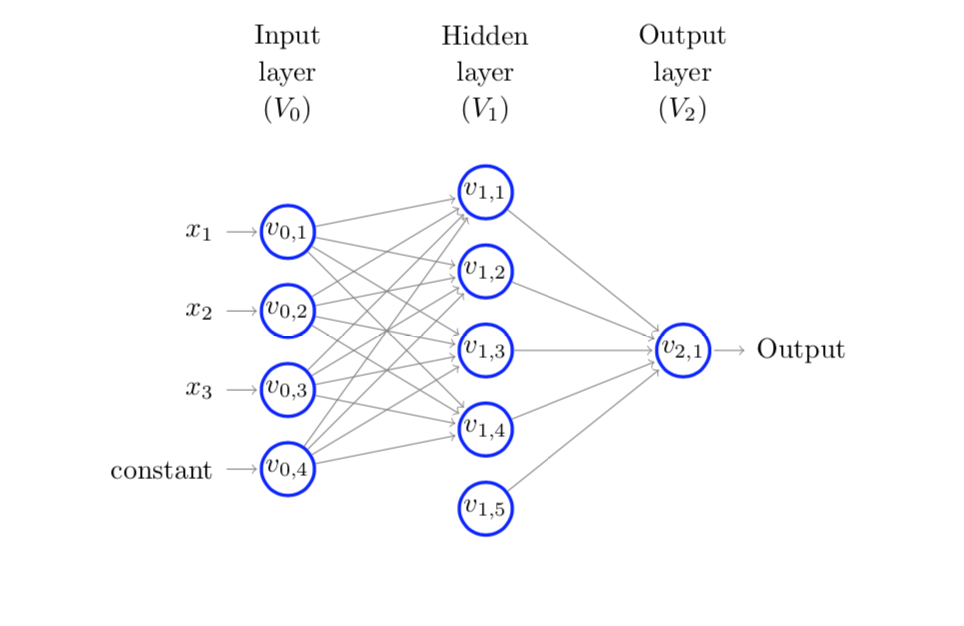
\includegraphics[width=\textwidth]{neural_network_example.png}
\caption{Neural Network architecture example, it has a 3-dimensional input layer
($V_0$), one hidden layer ($V_1$) and a single neuron output layer ($V_2$)
\cite{ShwartzUnderstadningML}.} 
\label{fig:neural_network_example}
\end{figure}

Starting from the tuple $(G, \sigma)$, often called the \emph{architecture of the network}, we can define the class of predictors: 
\[ \mathcal{F}_{G, \sigma} = \{ f_{G, \sigma, w} \mid w \textrm{ is a mapping from } E \textrm{ to } \mathbf R \} \]
From an expressiveness standpoint, it is proved that with a FNN using a binary input $x \in \{-1, 1\}^d$ and $\mathrm{sign}$ as activation
function $\sigma$, a single hidden layer network is able to
implement every binary function $f: \{-1, +1\}^d \to \{-1, +1\}$. Note that in practical term the binary constraint is just a useful simplification because a bit string of length $b$ represents every real coordinate in a computer.  That is, a single hidden layer is
enough to represent every Boolean function. The downside is that
the number of neurons required must be exponential in the dimension
of the input space. Currently, there are no mathematical proofs about the construction of
best network architecture for a given problem, nevertheless there is empirical evidence
about the fact that is better a network with fewer neurons distributed in many layers (deep
learning) rather than many neurons in a single layer. % TODO: citations

To train the weights of a feed-forward neural network is usually
used a gradient descent algorithm. The most common is called
Stochastic Gradient Descent (SGD). For every randomly sampled
example $x_t$ from the training set, the parameters $w(i, j)$ of the
network are updated using the following rule:
\begin{equation} \label{eq:sgd} 
w(i, j) \leftarrow w(i, j) -  \eta_t \frac{\delta\ell_{x_t}(W)}{\delta w(i, j )}
\end{equation}
where $\ell_(.)$ is a convex loss function. SGD is not the only
gradient descent algorithm used. In fact, in order to
improve the convergence of the neural networks many others algorithms were introduced,
the most popular were \emph{mini-batch gradient descent}, \emph{nesterov}, \emph{adagrad}
\cite{RuderGDOpt}. 

An algorithm called \emph{back-propagation} is used to compute the
gradients of the losses with respect of the weights in SGD. Using the chain rule of derivation the algorithm compute the the gradient with a layer by layer backward iteration
\cite{HintonBackProp}.
 

\section{Multi-Task Neural Networks}\label{sec:MTLsection}
%TODO: soft and hard parameter sharing figures
Multi-Task learning (MTL) is becoming increasingly popular in recent years.
Usually, to optimizing the predictions of a given task, a single model is
tuned and trained. In this way, good results can be achieved but, any
information that might come from related tasks are lost. MTL methods take
the signal from related considered tasks by sharing the
representation between them. The typical settings is to learning multiple
task simultaneously using a shared representation, what is learned by one
task can be helpful for the other tasks and vice versa \cite{Caruana97}. 
The mechanism underlining MTL, firstly described by \cite{Caruana97}, are reported in this Section.
There are many motivation behind MTL: from a biological point of view is
inspired by the way human brain learns (the knowledge of tasks can help us
learning other tasks), from a pure machine learning perspective
can be seen as a form of regularization in which the inductive bias is
introduced by the auxiliary tasks \cite{Ruder2017}. 

Multi-tasks learning introduce an \emph{implicit data augmentation}, that is, increase the sample size used to train the model. Furthermore, defining A and B as two related tasks with noise, learning A and B jointly gives a better representation due to the noise patterns averaging.
In addition, MTL permits the model to \emph{focus attention} on the feature that really matter. This behaviour, that could be considered as an implicit feature selection, is possible because other tasks could give additional evidence about relevance (or irrelevance) of features. 

MTL introduces the concept of \emph{eavesdropping}. The idea, introduced using hints by \cite{AbuMostafa1990}, is that we can allow the model to learn a features subset G, that is harder to learn from A, using another task B. 

In many cases, MTL permits to easily generalize to new future tasks. In fact, an hypothesis space that perform well for a large number of tasks will probably perform well for new tasks from the same environments \cite{Ruder2017}. 

While in the past MTL
was more used in non-neural models, recently many deep learning algorithms exploiting this approach were developed. We will briefly describe the two main ideas that have been pervasive in non-neural MTL models and then we will explain the neural networks approach.

The first important concept in MTL non-neural model is \emph{block-sparse regularization}. Consider $T$ tasks. Every tasks $t$ have a model $m_t$ with  a$d$-length parameters vectors $a_t$: 
\begin{equation}
a_t = \begin{bmatrix}
           a_{1, t} \\
           a_{2, t} \\
           \vdots \\
           a_{d, t}
         \end{bmatrix}^\mathsf{T}
\end{equation}
using these vectors we can form a matrix $A \in \mathbf{R}^{d \times T}$ stacking it columns by columns. Note that the rows of the matrix are the features considered while the columns are the models. Many works aimed to generalize the concept of regularization over the entire matrix $A$. For instance calculating $\ell_q$ norm for every rows and then compute $\ell_1$ norm over the obtained vector \cite{Ruder2017, Zhang2008, ArgyriouPontil2008, YuanLin2006}.  

The models just described assume a strong relation between the tasks. However, in a real worlds scenario, some tasks could not be closely related each others. Sharing information between unrelated tasks could lead the negatively the performance of the model, this phenomenon is often called \emph{negative transfer}. 
Many methods were introduced to overcome negative transfer. \cite{Evgeniou2005}, for instance, impose a clustering constraint that penalizing the norm and and the variance of our task columns vector.

In this context, the two
most used ways to perform multi-task learning are called \emph{soft
parameters sharing} and \emph{hard parameter sharing}. In the former
every task has his own set of parameters, the distance between this
parameters is regularized in order to become similar and represent
multiple tasks. Notable examples are \cite{duong-etal-2015-low} and
\cite{yang2016trace}. In the latter instead, a fixed number of hidden
layers are shared between tasks and keeping several task-specific output
layers. In this works, we have focused on hard-parameters sharing methods
to implement our MTL networks. Given $N$ the number of tasks, it is proved
that hard-parameters sharing reduce the risk of over-fitting $N$ times
compared to task-specific models \cite{baxter1997}.
\begin{figure}
\centering
\begin{subfigure}{.5\textwidth}
  \centering
  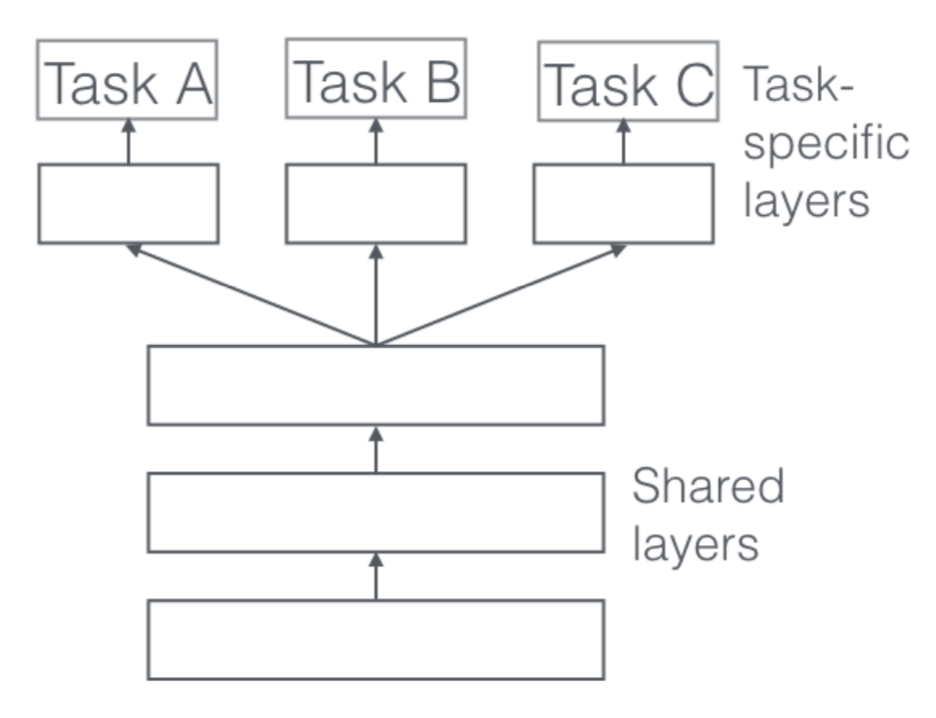
\includegraphics[width=.7\linewidth]{MTL_hard.png}
  \label{fig:sub1}
\end{subfigure}%
\begin{subfigure}{.5\textwidth}
  \centering
  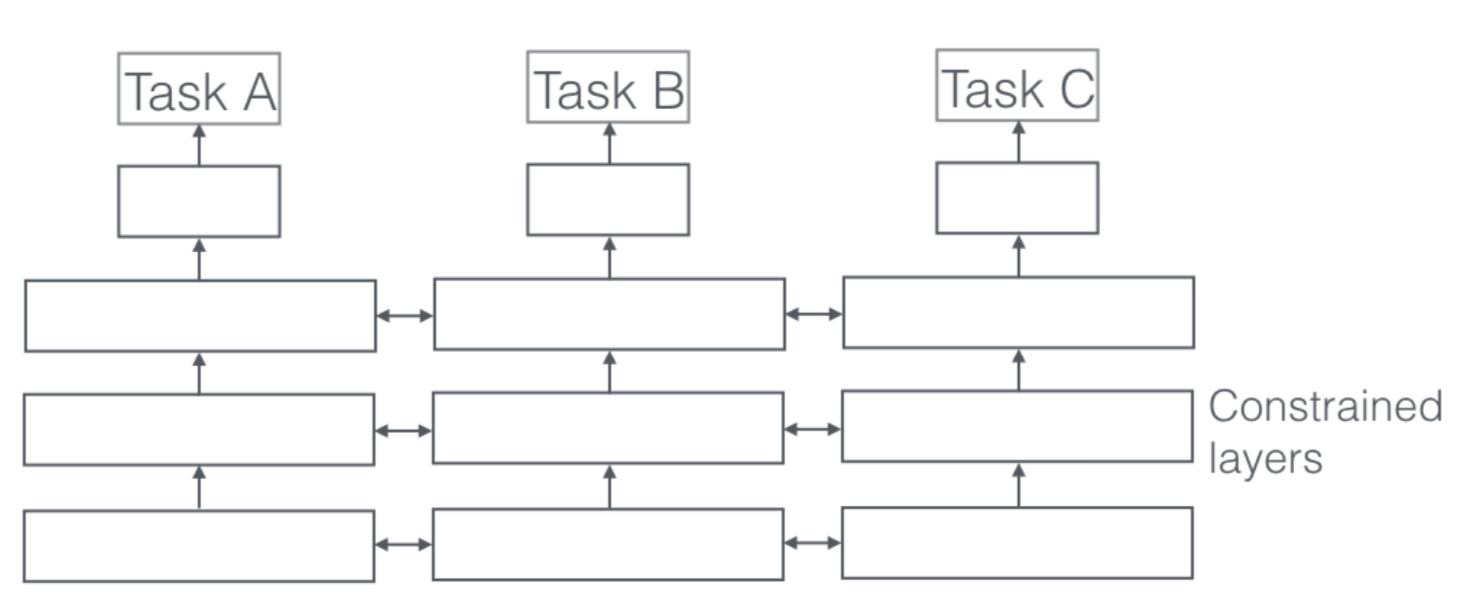
\includegraphics[width=1.2\linewidth]{MTL_soft}
  \label{fig:sub2}
\end{subfigure}
\caption{Hard parameter sharing, on the left, and soft parameter sharing, on the right, for multi-task learning in deep neural networks.}
\label{fig:test}
\end{figure}

As already mentioned, soft and hard parameters sharing are the two main used MTL methods in deep learning. Despite this, many works tried to develop better mechanisms for MTL in deep neural networks. Among them we can mention deep relationship networks \cite{NIPS2017_6757}, fully-adaptive feature sharing \cite{fullyadaptive}, cross-stitch networks \cite{crossstichnet}, low supervision \cite{sogaard-goldberg-2016-deep}, joint many-task model \cite{hashimoto-etal-2017-joint}, weighting losses with uncertainty \cite{Kendall}, tensor factorization for MTL \cite{Yang2017DeepMR} and, finally, sluice networks \cite{Ruder2017SluiceNL}.

\section{Gaussian Process for Hyper-parameters Tuning of the Models}
\label{sec:gaussianprocess}
% todo: integrate
% todo: read again
% todo: images
% todo: fix mathematical formalization (???)
In Section~\ref{sec:singletaskNN} and Section~\ref{sec:MTLsection} we
described the theoretical aspects of training single-task and multi-task neural networks. In practical terms, due to the
growing complexity of deep learning models, working with neural networks
involves a proper choice of many hyperparameters, such as the shape of
the network architecture, the learning rate, or the regularizer weight
decay. Over the years, many hyper-parameters optimization algorithms were
proposed. Among this, grid and random search \cite{BergstraB12} are significant examples. A more sophisticated model could be exploiting Bayesian optimization
and use it to choose the best hyper-parameters for a given model
\cite{SnoekGP}. In general, optimizers aim to minimize (or
maximize) a scoring function respect its hyper-parameters, given
$\mathcal{X}$ the set of hyper-parameters and $f(x)$ the scoring function of interest
(i.e., auPRC, auROC, rmse, binary loss etc.) we have: 
\[ 
x^* =  \argmin_{x \in \mathcal{X}} f(x) 
\]
the main difference between Bayesian optimization in comparison with more
traditional approaches is that Bayesian optimization chooses the next
hyper-parameters set in an informed way. It keeps track of past evaluations
that use to build a probabilistic model called \emph{surrogate function}. This function is often built using a Gaussian process. That is, in every
iteration the surrogate function is updated selecting, with a particular
\emph{selection function} (i.e., Expected Improvement function), and
evaluating a new set of hyper-parameters. On one hand Bayesian methods
take more time smartly choosing the next set of hyper-parameters, on the other hand they make few iterations in total compared to grid and random search. 
Recently Keras developer has released a new hyperparameter optimizer
open-source library called Keras-tuner \footnote{Available on GitHub:
\url{https://github.com/keras-team/keras-tuner}}
\cite{omalley2019kerastuner}. It contains, among many others, an
implementation of Bayesian optimization\footnote{Documentation available
at: \url{https://keras-team.github.io/keras-tuner/documentation/tuners/}}.

\section{Evaluation Metrics} \label{sec:methods_metrics}
In this section the principal evaluation metrics used in this work are described. 
In Section~\ref{sec:singletaskNN} we described Stochastic Gradient Descend algorithm. In order to update the parameters of the network in Equation~\ref{eq:sgd} we have seen that we need to calculate the derivative of a convex loss function $\ell(.)$ with respect to the weights. In this work, in order to train both single and multi task neural networks, we utilized a well-known loss function, often used in binary classification, called \emph{binary cross-entropy}. Given $t \in \{0, 1\}$, the true binary label of a sample, and $s \in [0\..1]$, the probability score given by a predictor, we define binary cross-entropy as:
\begin{equation}
    \ell(t, s) = -t\log(s) - (1 - t)\log(1 - s)
\end{equation}
In order to evaluate the performance of the models, many metrics can be used. Despite its simplicity, one of the most popular is \emph{Accuracy} defined as the proportion of the correct respect the total number of sample
\begin{equation}
    \textrm{accuracy} = \frac{\#\{\textrm{correct samples}\}}{\#\{\textrm{total samples}\}}
\end{equation}
It is easy to notice that the main drawback of accuracy is that, with an unbalanced dataset, we can achieve misleading higher values. Fortunately, during the years, more stable performance evaluation metrics were introduced in order to overcome accuracy disadvantages. In the contest of binary classification, before describing these new metrics, we must introduce four classification terms: 
\begin{itemize}
\item \emph{True Positive} (TP): samples classified as positive where also the actual value are positive;
\item \emph{False Positive} (FP): samples classified as positive where the actual values are negative;
\item \emph{True Negative} (TN): samples classified as negative where also the actual values are negative;
\item \emph{False Negative} (FN): samples classified as negative where the actual values are positive.
\end{itemize}
Of course, a good model aims to have a very high rate of true positive and true negative. From this point of view, to evaluate the goodness of a model we can use \emph{precision} and \emph{recall}. Precision evaluate the ability of a model to classify relevant results correctly 
\begin{equation}
    \textrm{precision} = \frac{\textrm{TP}}{\textrm{TP}+\textrm{FP}}
\end{equation}
recall, instead, is the percentage of total relevant results correctly classified by the algorithm 
\begin{equation}
    \textrm{recall} = \frac{\textrm{TP}}{\textrm{TP}+\textrm{FN}}
\end{equation}
this two metrics are often put together computing the harmonic mean between them, obtaining a new metric called \emph{F1-score}:
\begin{equation}
    \textrm{F1-score} = 2 \cdot \frac{\textrm{precision} \cdot \textrm{recall}}{\textrm{precision}+\textrm{recall}}
\end{equation}
Finally, we describe the two main metrics used to evaluate the performance of the models used in this work: \emph{Area Under the Receiver Operating Characteristics} (auROC) and \emph{Area Under the Precision-Recall Curve} (auPRC). 
The auROC is computed plotting the ROC curve with Recall on y-axis against False Positive Rate (FPS) on x-axis and calculating the area under it.  Similarly, auPRC is computed plotting precision on y-axis against recall on x-axis and calculating the area under it. Since both precision and recall does not consider true negative sample, auPRC is used when having good performance on negative example are not extremely important. 

\chapter{Dataset}
\section{Epigenetic Data} \label{sec:epigenomic_data}
%scrivere qualcosa di più sui dati epigenomici (cosa sono?)
In order to train and compare our single-tasks and multi-tasks neural networks explained in Chapter~\ref{cap:methods} we built a dataset of epigenetic data. We gathered the epigenetic features data from
ENCODE \cite{ENCODE_data} and the enhancers and promoters labels from
FANTOM \cite{FANTOM_data}. Formally we can define our data as follow: 
\begin{itemize}
    \item $L$ is the set of \emph{cell lines};
    \item $C$ is the set of \emph{chromosomes};
    \item $I$ is the set of \emph{intervals} over the natural numbers;
    \item $S_\ell\subseteq C\times I$, $\ell\in L$, is the set of \emph{sequences} (pair of chromosomes and intervals) relative to the cell line $\ell$, which can be mapped injectively to sequences of 1000; in general, $S_\ell\neq S_{\ell'}$; the mapping to the nucleotides is dependent on the pair chromosome/interval only;
    \item $Y$ is the set of \emph{labels} from FANTOM that can be associated to sequences (e.g., active promoter);
    \item for each $\ell\in L$, $F_\ell$ is a set of \emph{features} and $e_\ell:S_\ell\to\mathbf R^{F_\ell}$ is a map representing ENCODE \emph{epigenetic data};
\end{itemize}
%TODO: check cell lines description correctness 
The set of cell lines $L$ includes: 
\begin{description} 
\item A549 a lung carcinoma cell line derived from old Caucasian male;
\item GM12878 a lymphoblastoid cell line produced from the blood of a female donor with northern and western European ancestry by EBV transformation;
\item H1 an human embryonic stem cell line; 
\item HEK293 a human embryonic kidney cell line;
\item HEPG2 a cell line derived from a male patient with liver carcinoma;
\item K562 an immortalized cell line produced from a female patient with chronic myelogenous leukemia;
\item MCF7 a mammary gland adenocarcinoma cell line.
\end{description}
For every cell lines $\ell \in L$, the set of sequences $S_\ell$ contains the genomics locations of enhancers and promoters. $Y$ contains the four classes of labeled regions, including \emph{active enhancers} (A-E), \emph{active promoters} (A-P), \emph{inactive enhancers} (I-E), \emph{inactive promoters} (I-P). A-E and I-E labels are defined as FANTOM enhancers with $TPM>0$ (tags per million) and $TPM=0$, respectively. A-P and I-P labels, instead, are promoters with $TPM>5$ and $TPM=0$. 
% Todo: Ultima frase presa da spiegazione di paper wasserman, cos'è TPM?! lo spiego?

%TODO: sistemare con riferimenti per uso media e mediana per l'imputer
For every cell line $\ell \in L$, the number of features $| F_\ell |$ are reported in Table~\ref{tab:featuressize}. It can be noted that, some cell lines, such as K562, HepG2 and HEK293 contains more than 200 features. In Section~\ref{sec:featureselection} we reported the approach followed to select a subset of discriminative features.
Note that, for every cell lines $\ell \in L$, in vitro experiments are
performed for every nucleotides of sequences. Consequently the pure ENCODE
data, for every sequence $s \in S_\ell$ and epigenomic feature $f \in
F_\ell$ (e.g., POLR2A), are represented by a $|s|$-length vectors of real
numbers. Those values must be summarized in a single metrics. The most
common used metrics are mean, variance and maximum, we choose to use
maximum. Moreover we have a very small percentage (less than 1\%) of
missing values; thus, we used as substitute the median of the others
values.
\begin{table}[t]
\centering
\begin{tabular}{|l|l|l|}
\hline
\textbf{Cell lines ($\ell \in L$)} & \textbf{$|F_\ell|$} & \textbf{$|F_\ell^{i^{*}}|$} \\ \hline
A549               & 54 & 14                  \\ \hline
GM12878            & 110 & 38                 \\ \hline
H1                 & 43 & 20                  \\ \hline
HEK293             & 207 & 35                 \\ \hline
HepG2              & 209 & 21                 \\ \hline
K562               & 320 & 36                 \\ \hline
MCF7               & 101 & 19                 \\ \hline
\end{tabular}
\caption{Original feature set and number of features selected for every cell line in $L$ compared}
\label{tab:featuressize}
\end{table}
\section{Computational Tasks} \label{sec:computational_tasks}
To evaluate the performance of our models in discriminating the different cis-regulatory regions labels $Y$ we proposed a group of \emph{computational problems}. Given the set of labels $Y$, a computational problem is defined as a set of binary tuples $P \subseteq Y \times Y$; In particular $P$ contains the following tuples: 
\begin{itemize}
    \item Active Enhancers vs Active Promoters (A-E vs A-P);
    \item Active Promoters vs Inactive Promoters (A-P vs I-P);
    \item Active Enhancers vs Inactive Enhancers (A-E vs I-E); 
    \item Inactive Enhancers vs Inactive Promoters (I-E vs I-P); 
    \item Active Enhancers and Active Promoters vs Background (A-E+A-P vs BG).
\end{itemize}
In terms of classification, we considered the first and the second element of every items as the positive and negative training classes. For instance, A-E and A-P are considered as positive and negative example, respectively. The last item is built by joining in positive class A-E and A-P labels and in negative class all the other labels. In other terms BG is composed by I-E and I-P labels. The performance of every computational problems are evaluated for every cell line $\ell \in L$. Thus we define a \emph{tasks} as a pair $p \in P \times L$. 

\section{Feature Selection} \label{sec:featureselection}
As previously described, in the problem at the hand we have different set of epigenomic features $F_\ell$ for every cell line $\ell \in L$. As shown in Table~\ref{tab:featuressize}, some cell lines have a considerable size set of features, so many features might arise to a performance degradation of the models due to, for instance, to over-fitting. During the years many methods were developed to deal with large dimensional features sets. Iz this section we provide a detailed explanation of the feature selection approach followed in this work and the results it produced. 

Firstly, we tried to understand, for every cell lines, the number of features to select. To do this we use a well-known algorithm called Recursive Feature Elimination (RFE) \cite{VapnikRFE}. Given a model that assign weights to the features, RFE use them to recursively remove the least important feature until the last one. In this way, for every iterations $i$, we obtain a subset of features $F_{\ell}^{i} \subseteq F_\ell$. Note that the obtained subset are nested, $F_{\ell}^{1}  \subseteq  F_{\ell}^{2} \subseteq \cdots \subseteq F_{\ell}$. In order to obtain more accurate results, every RFE run is cross-validated. For every tasks $p \in P \times L$ and for every feature subset $F_\ell^i$ we computed the \emph{f1-score} function values against the number of best features. The performance of the model should increase with the increasing of the best features selected until a certain limit the best number of feature and reach a plateau or in some cases decrease. The maximum of the function can be considered the optimal number of feature to select. Thus, given $i^{*}$ the index of the best subset iteration, the optimal number of feature $|F_\ell^{i^{*}}|$ for a certain task could be selected looking at the maximum of this function. In Figure~\ref{fig:feats_plot} we report the obtained results, every plot consider a cell lines and every curve is a particular task $p$, the colored dotted vertical lines indicate respectively the maximum \emph{f1-score} for a given task. The black vertical line, instead, is the average number of feature between every computationl problem. 

After fixing the number of features that should be considered for every cell lines (Table~\ref{tab:featuressize}) we tried to understand which features must be selected. Many methods could be found in literature in order to choose an optimal subset of features of given size. They are mainly divided into: \emph{filters} methods that rank features computing correlation coefficients and \emph{wrapper} methods that use models to score subsets of features \cite{Guyon}. Every approach has its own advantages, in order to have a proper feature selection we choose to join some selected approaches together, in particular:
\begin{itemize}
    \item \textit{Correlations with target}: it is a filter based method. Pearson correlation is computed for every features $f \in F_\ell$ against the target labels. The correlations values are used to ranking the features;
    \item \textit{Random Forest Wrapper}: the features are ranked using the \emph{Gini importance} \cite{giniimportance} of the features calculated during the training of a Random Forest \cite{breiman2001random}; 
    \item \textit{Logistic Regression Wrapper}: similar to the Random Forest Wrapper but the features are ranked using the coefficient of the features in the decision function of a trained Linear Regressor.
    \item \emph{Recursive Feature Elimination}: in addition to using RFE for selecting the optimal number of features, we also used it to select an optimal subset of given dimension. 
\end{itemize}
For every cell lines $\ell \in L$ and every task $p \in P$ we build a binary matrix $I_\ell(|F_\ell|, 4)$, which have the features on the rows and the described selection methods on the columns. For every rows $f$ and every columns $m$ the element $i_{fm}$ of $I$ is defined as follow: 
\[
    i_{fm} = \begin{cases} 1 & \mbox{if } f \mbox{ is selected by method } m \\ 0 & \mbox{otherwise} \end{cases}
\]
the number of ones in every rows $f$ give us a measure of the importance of each feature. The obtained values are averaged for every tasks $p \in P \times L$. 
% TODO: put results in appendix?!

\begin{figure}[!htb]
    \centering
    \begin{subfigure}[b]{0.48\textwidth}
        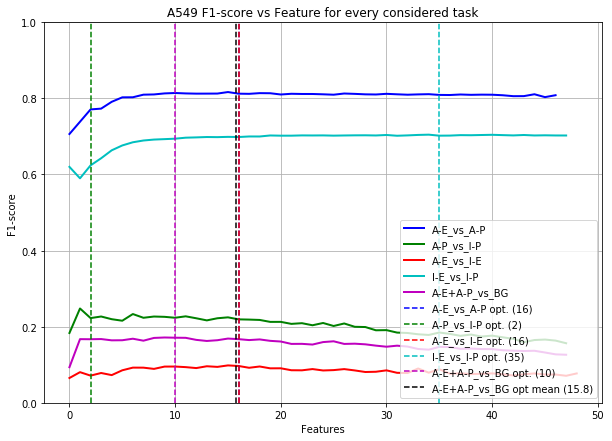
\includegraphics[width=\textwidth]{images/features_plots/A549_feature_plot.png}
        \caption{A549}
        \label{fig:A549_n_feat}
    \end{subfigure}
    ~ 
    \begin{subfigure}[b]{0.48\textwidth}
        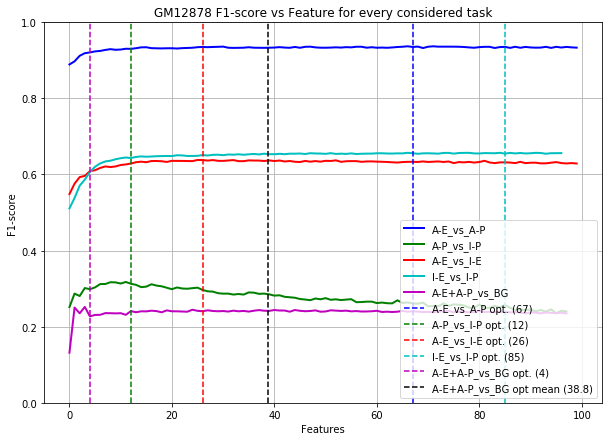
\includegraphics[width=\textwidth]{images/features_plots/GM12878_feature_plot.png}
        \caption{GM12878}
        \label{fig:GM12878_n_feat}
    \end{subfigure}
    ~ 
    \begin{subfigure}[b]{0.48\textwidth}
        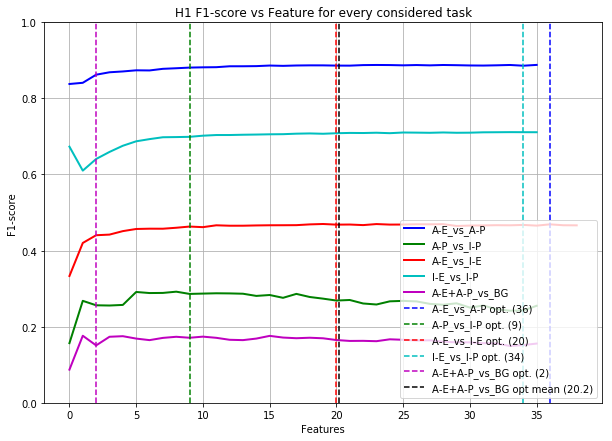
\includegraphics[width=\textwidth]{images/features_plots/H1_feature_plot.png}
        \caption{A mouse}
        \label{fig:H1_n_feat}
    \end{subfigure}
    \begin{subfigure}[b]{0.48\textwidth}
        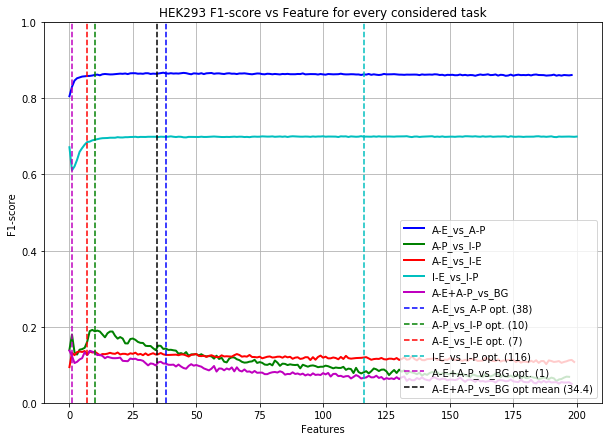
\includegraphics[width=\textwidth]{images/features_plots/HEK293_feature_plot.png}
        \caption{HEK293}
        \label{fig:HEK293_n_feat}
    \end{subfigure}
    
    \begin{subfigure}[b]{0.45\textwidth}
        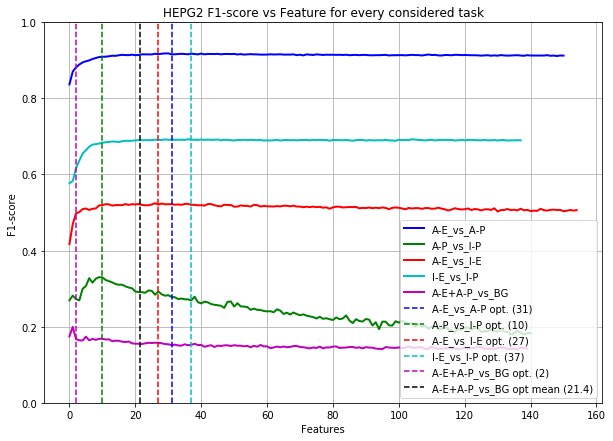
\includegraphics[width=\textwidth]{images/features_plots/HEPG2_feature_plot.png}
        \caption{HEPG2}
        \label{fig:HEPG2_n_feat}
    \end{subfigure}
    \begin{subfigure}[b]{0.48\textwidth}
        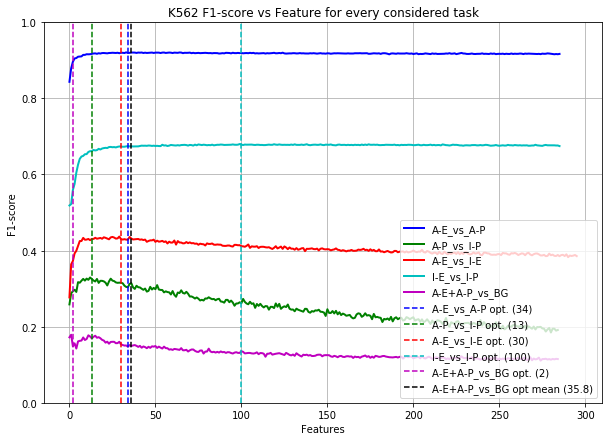
\includegraphics[width=\textwidth]{images/features_plots/K562_feature_plot.png}
        \caption{K562}
        \label{fig:K562_n_feat}
    \end{subfigure}
    
    \begin{subfigure}[b]{0.48\textwidth}
        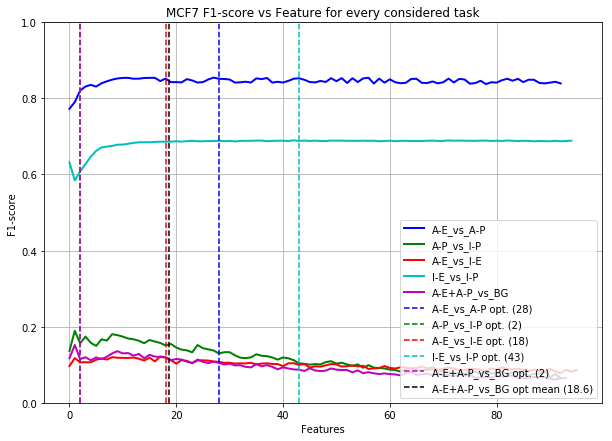
\includegraphics[width=\textwidth]{images/features_plots/MCF7_feature_plot.png}
        \caption{MCF7}
        \label{fig:MCF7_n_feat}
    \end{subfigure}
    \caption{Accuracy vs Number of Features plots for every $\ell in L$}\label{fig:feats_plot}
\end{figure}


\section{t-SNE Decomposition}
In order to have a general idea of the points separability we tried to  project them in a 2-dimensional space. Among many dimensionality reduction algorithm t-SNE were chosen. t-Distributed Stochastic Neighbor Embedding (t-SNE) \cite{vanDerMaaten2008} is an improvement of standard SNE \cite{HintonSNE} that allow a better cost function optimization. So, for every given task $p$, we  computed the t-SNE of every cell lines. 
In Appendix~\ref{appendix:tsne} we report the results of analysis, every figure is a computational problem and every plot is a cell line $\ell$. We can notice that with the exception of A-E vs A-P (Figure~\ref{fig:tsneAEvsAP}) and A-E+A-P vs BG (Figure~\ref{fig:tsneAE+APvsBG}), respectively the least and the most numerous computational problems, all the other plots highlight evident clusters between positive (in blue) and negative (in red) labels. 

\chapter{Experimental Setup}
% general setup (train test splitting etc.)
% balanced unbaanced
\section{General Experiments Configuration}
\label{sec:exp_setup_general}
As explained before the aim of this work is comparing the  cis-regulatory regions classification capabilities of two deep learning models: single-task and multi-task neural networks. Although the considered experiments have different setups, described in details later (Section~\ref{sec:exp_setup_singletask} and Section~\ref{sec:exp_setup_multitask}), in this Section we explain their common traits. 

The two models are trained and evaluated for every computational task $p \in P \times L$ described in Section~\ref{sec:computational_tasks}. 
To validate and generalize the results of our
models we used a holdout method. In particular, every experiment uses ten external holdouts and one internal
holdout. Basically, for every external
holdout, the dataset is split in \emph{training} and \emph{test} sets, the
training set is further partitioned in \emph{internal training} and validation
sets. Internal training and validation set are used by the Gaussian Process to
choose the optimal set of hyper-parameters (Section~\ref{sec:gaussianprocess}).
The best model found is retrained using the full training set (internal training + validation) and evaluated using the test set. This procedure is
repeated 10 times and the final performance metrics are obtained averaging auPRC
and auROC of every external holdout (see Section~\ref{sec:methods_metrics}). The proportion between internal and external holdouts samples are respectively 70\% and 30\%. In Figure~\ref{fig:train_test_diagram} we show a diagram of one (out of ten) external and internal holdouts process. 
\begin{figure}[ht]
\centering
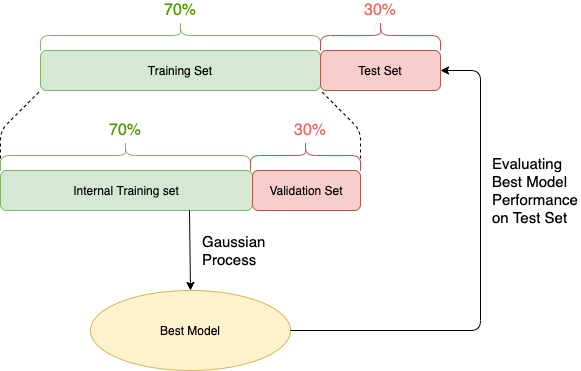
\includegraphics[width=0.9\textwidth]{train_test_scheme.png}
\caption{Single internal and external holdouts process diagram. Note that this
process is repeated 10 times.} 
\label{fig:train_test_diagram}
\end{figure}
In order to train both single-task and multi-task models, we used the data described in Section~\ref{sec:epigenomic_data}. The features are filtered using the selection methods described earlier (see Section~\ref{sec:featureselection}). In Appendix~\ref{appendix:features_tables} are reported the tables containing the selected features. 
Furthermore, for both models, we tried to use both an unbalanced and balanced configurations of training and test sets. 

\section{Single-Task Neural Network Architecture} 
\label{sec:exp_setup_singletask}
% single task neural network setup
To evaluate the performance of multi-task neural networks, we need to consider a benchmark model in our experimental setup. Due to their excellent results, obtained in the context of CRRs classification \cite{WassermannDECRES}, we choose to use a classical feed-forward neural network (explained in Section~\ref{sec:singletaskNN}). Fixed a computational task $p$, the network takes the reduced set of epigenetic features as input and gives the prediction of the labels $Y$. A Gaussian process performs the model search. The models can have no hidden layers up to three hidden layers. In Table~\ref{tab:mlp_single_arch} are reported the number of neurons search space for every layer of the network. Since we have seen in previous experiments that pyramidal architecture networks give better performances the bayesian optimizer is always forced to select an architecture such as the neurons of layer $i$ are greater or equals to the neurons of layer $i+1$. 
A slight variation of SGD explained in Section~\ref{sec:singletaskNN} called Stochastic Gradient Descend with momentum is employed to optimize the weights of the network. The initial learning rate, the $\ell_2$-regularization amount to control model complexity, and the momentum to stabilize the optimization are set respectively to 0.3, 0.001 and 0.5. The training set is iterated for 1000 epochs maximum, and the learning rate could be reduced as the number of iterations increases with a rate of 0.01. Finally, the batch size is fixed at 100 samples per batch.  
\begin{table}[t]
\centering
\begin{tabular}{lll}
\toprule
\textbf{Layer} & \textbf{Neurons} & \textbf{Activation} \\ 
\midrule
1 & (2, 4, 8, 16, 32, 64, 128, 256) & ReLU \\ 
2 & (2, 4, 8, 16, 32, 64, 128) & ReLU \\ 
3 & (2, 4, 8, 16, 32, 64) & ReLU \\ 
4 & 1 & Sigmoid \\ 
\bottomrule
\end{tabular}
\caption{Parameters setting for single-task feed-forward neural network}
\label{tab:mlp_single_arch}
\end{table}

The code implementing the single-task experiments was originally developed in University of Milan by a Computational Biology and Bioinformatics laboratory (Anacleto Lab) research group in order to evaluate the ability of neural networks to distinguish cis-regulatory regions. Some of those experiments have been repeated and the results are discussed in Section~\ref{sec:single_results}. 

\section{Multi-Task neural network architecture} \label{sec:exp_setup_multitask}
% multi task neural network setup
We choose to use an hard parameters sharing architecture explained in Section~\ref{sec:MTLsection}. The model is constructed with a multi-input and multi-output setting. There is an input branch for every feature set $F_\ell$ and an output branch for every cell line. The main body of hidden layers connects input branches with output branches. Summarizing the architecture is divided into the following three main parts:
\begin{itemize}
    \item \textit{input branches layers}: every $F_\ell$ will be taken in input by a different branch of hidden layers;
    \item \textit{main body}: it is composed by shared hidden layers. These hidden layers aim to share knowledge between cell lines. The prediction on a particular line $\ell$ could be affected by the information given from the other ones;
    \item \textit{output branches layers}: the main body is split in different branches of hidden layers. Their purpose is giving the predictions of labels $Y$ of every $\ell \in L$.
\end{itemize}
In Figure~\ref{fig:MTL_arch_diagram} we report a diagram of the used architecture. Every input branch is fully connected with the main body. That is, every neuron belonging to the last layer of input branches is connected with every node of the main body first layer. The main body and the output branches have the same type of connection. Finally, the output of the network is calculated using a sigmoid function. 
\begin{figure}[ht]
\centering
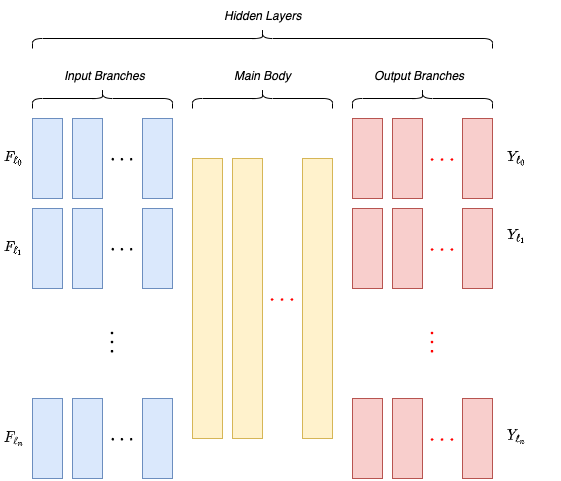
\includegraphics[width=\textwidth]{MTL_diagram.png}
\caption{Multi-tasks neural network architecture. On the left, every input branch takes a cell lines feature set, on the right, every output branch gives the predictions for every cell line $\ell$. They are connected, in the middle, by the main body layers. } 
\label{fig:MTL_arch_diagram}
\end{figure}
Note that the network could have the input or the output directly connected to the main body without any input or output layers. 
Also in this case, the model search is performed by the Gaussian Process
(Section~\ref{sec:gaussianprocess}). The input branches, output branches and
the main body can have from zero up to three layers. In Table~\ref{tab:mplmtl} are summarized the number of neurons search space for every part of the network. 
To train the models, a Stochastic Gradient Descent with momentum algorithm is used. The initial learning rate is chosen by Gaussian optimizer in a range between 0.1 and 0.2 and it decays with the increasing of iterations with a 0.01 rate. The momentum and the dropout (a form of model complexity control) are set respectively to 0.5 and 0.2. Also in this case, the model is iterated for 1000 epochs, the batch size is fixed to 1000 sample per batch. 
\begin{table}[t]
\centering
\begin{tabular}{llll}
\toprule
\textbf{Arch. Parts} & \textbf{Layers} & \textbf{Neurons per Layer} & \textbf{Activation} \\ 
\midrule
\multirow{2}{*}{\textit{Input branch}}  & 1 & 64, 128, 256, 512 & ReLU \\ 
{} & 2 & 32, 64, 128, 256, 512 & ReLU \\
{} & 3 & 16, 32, 64, 128, 256, 512 & ReLU \\
\midrule
\multirow{2}{*}{\textit{main body}} & 1 & 2, 4, 8, 16, 32, 64, 128, 256, 512 & ReLU \\ 
{} & 2 & 2, 4, 8, 16, 32, 64, 128, 512 & ReLU \\
{} & 3 & 2, 4, 8, 16, 32, 64, 128, 256, 512 & ReLU \\
\midrule
\multirow{2}{*}{\textit{output branch}} & 1 & 2, 4, 8, 16, 32, 64, 128, 256, 512 & ReLU\\ 
{} & 2 & 2, 4, 8, 16, 32, 64, 128, 256, 512 & ReLU \\
{} & 3 & 2, 4, 8, 16, 32, 64, 128, 256, 512 & Sigmoid \\
\bottomrule
\end{tabular}
\caption{Parameters setting for multi-task neural network}
\label{tab:mplmtl}
\end{table}
For all of the three parts just described, we tried two neurons size configurations. In the former we constrained the Gaussian process to keep a fixed number of neurons for every layer, in the latter, instead, for every neural network section (input branches, main body, output branches) the optimizer selects a pyramidal structure where the neurons of layer $i$ are greater or equals to the neurons of layer $i+1$.
In Section~\ref{sec:multi_results} we reported the results obtained from the various experiments configurations. 

The code implementing these experiments has been developed by the authors of this work in a collaboration between the Laboratory for Web Algorithmics (LAW) and Computational Biology and Bioinformatics laboratory (Anacleto Lab) in the University of Milan. This code is available on Github\footnote{\url{https://github.com/lipry/MultiTaskLearningExperiments}}. The obtained results are discussed in Section~\ref{sec:multi_results}.



\chapter{Results}
\section{Single-Task Neural Networks Results}
\label{sec:single_results}
In this Section we report the results obtained using single-tasks neural networks. Since this deep learning model is considered state-of-the-art in CRRs classification, we use these experiments as a benchmark for evaluating the performance of multi-task neural networks (Section~\ref{sec:multi_results}). The experiments are performed with the experimental setups described in Section~\ref{sec:exp_setup_general} and Section~\ref{sec:exp_setup_singletask}, the model are trained using the two set of features described in Section~\ref{sec:featureselection} 

Firstly, we discuss the results obtained training a single-task neural network using $F_\ell^{\textrm{acc}}$ as features set and without balancing the dataset. The bar plots in Figure~\ref{fig:unbalanced_old_results} report the average auROC and auPRC obtained, the same results are summarized in Table~\ref{tab:unbalanced_old_auroc} and Table~\ref{tab:unbalanced_old_auprc} in Appendix~\ref{appendix:results_tables}. Almost for every computational task, auROC is greater than 0.6. Despite this in some cases, such as A-P vs I-P and I-E vs I-P respectively in HEK293 and MCF7, the model obtained very low results. auPRC results instead are not very promising. In both average auROC and average auPRC results emerge that this model is very good in distinguish active enhancers from active promoters (A-E vs A-P) obtaining always values greater than 0.9.
\begin{figure}[!htbp]
    \centering
    \begin{subfigure}[b]{\textwidth}
        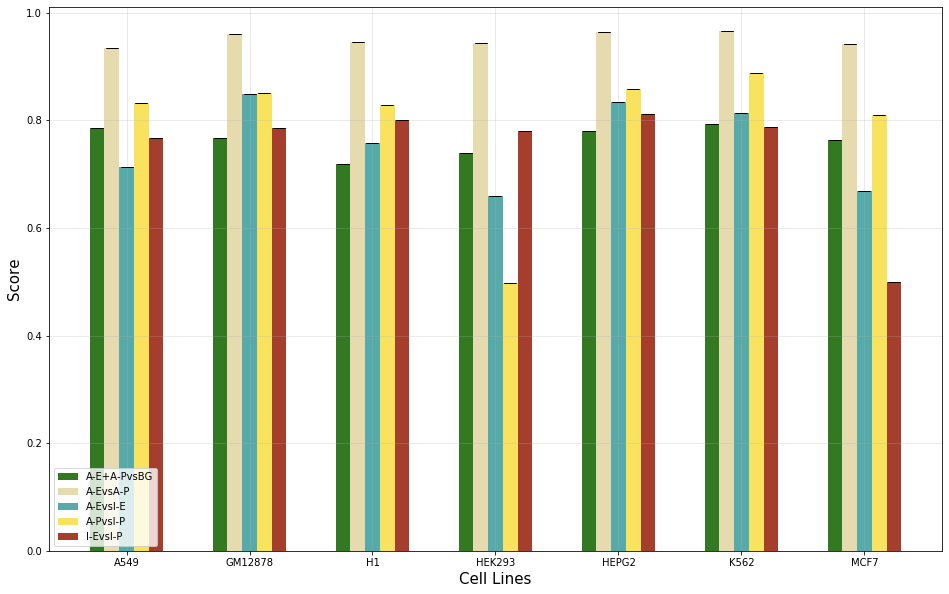
\includegraphics[width=\textwidth]{images/results_plots/single_tasks/unbalanced_old_auroc.png}
        \caption{auROC}
        \label{fig:auroc_unbalanced_old}
    \end{subfigure}
    \begin{subfigure}[b]{\textwidth}
        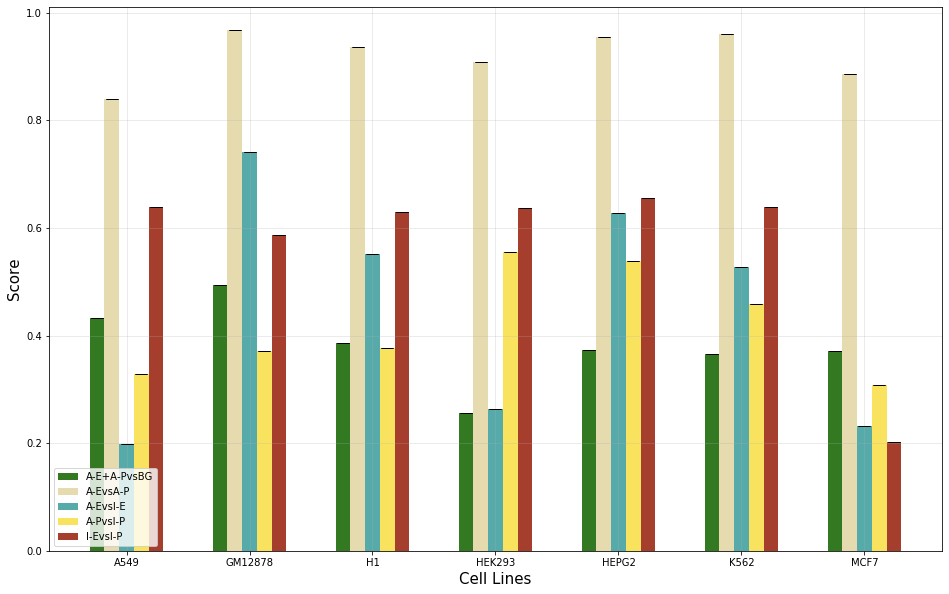
\includegraphics[width=\textwidth]{images/results_plots/single_tasks/unbalanced_old_auprc.png}
        \caption{auPRC}
        \label{fig:auprc_unbalanced_old}
    \end{subfigure}
    \caption{auROC and auPRC for single-task neural network trained using $F_\ell^{\textrm{acc}}$ as features and unbalanced dataset.}\label{fig:unbalanced_old_results}
\end{figure}

In order to improve the results of the model, using the same set of features $F_\ell^{\textrm{acc}}$, we repeated the experiment balancing both training and test set. Comparing Figure~\ref{fig:auprc_balanced_old}, containing the results with a balanced dataset, and Figure~\ref{fig:auroc_unbalanced_old}, containing the previous results with an unbalanced setting, we can notice an average auPRC improvement in almost every tasks $p$ of every cell lines $\ell \in L$. On the other hand the average auROC remains nearly unchanged (Figure~\ref{fig:balanced_old_results} and Figure~\ref{fig:unbalanced_old_results}). 

\begin{figure}[!htbp]
    \centering
    \begin{subfigure}[b]{\textwidth}
        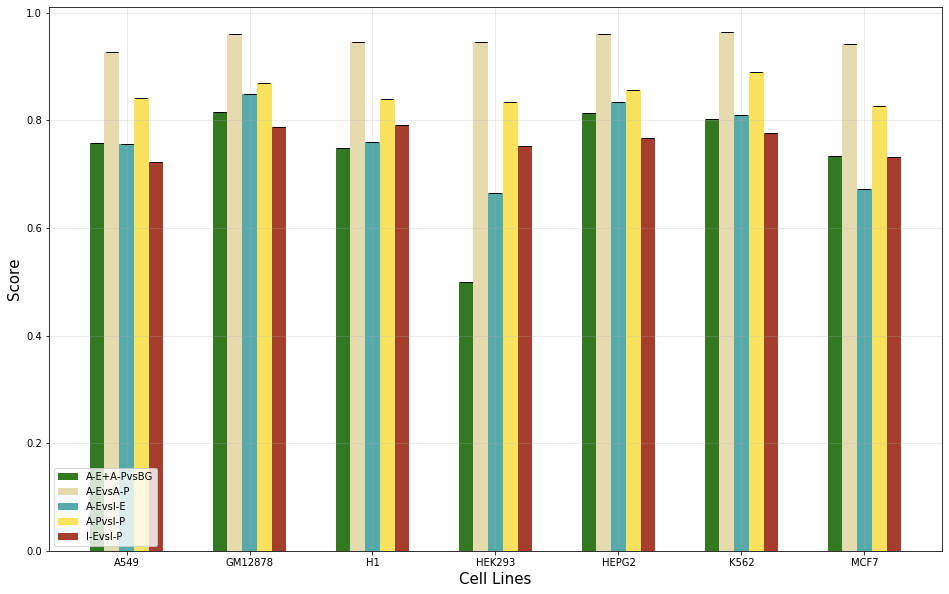
\includegraphics[width=\textwidth]{images/results_plots/single_tasks/balanced_old_auroc.png}
        \caption{auROC}
        \label{fig:auroc_balanced_old}
    \end{subfigure}
    \begin{subfigure}[b]{\textwidth}
        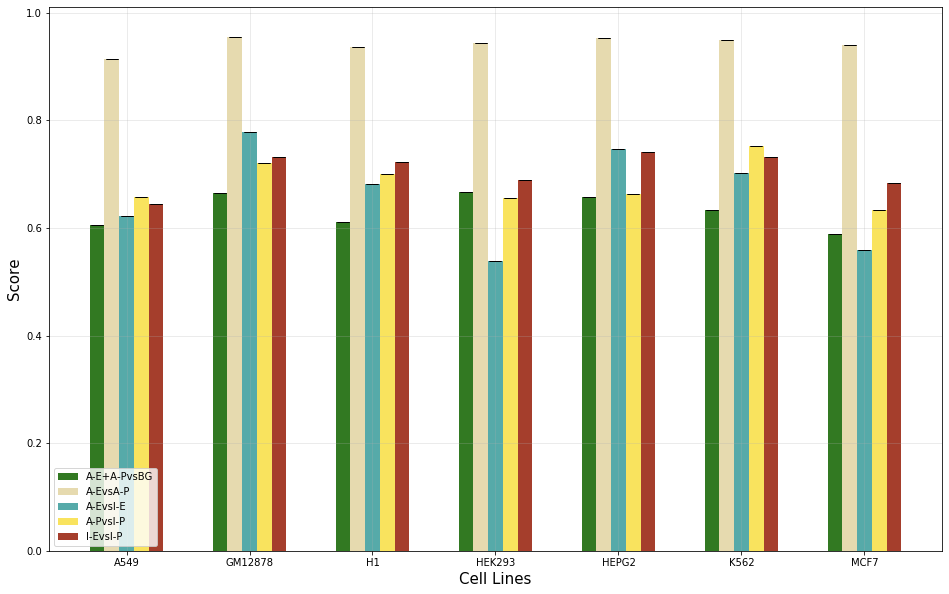
\includegraphics[width=\textwidth]{images/results_plots/single_tasks/balanced_old_auprc.png}
        \caption{auPRC}
        \label{fig:auprc_balanced_old}
    \end{subfigure}
    \caption{auROC and auPRC for single-task neural network trained using $F_\ell^{\textrm{acc}}$ as features and balanced dataset.}\label{fig:balanced_old_results}
\end{figure}

Finally, we repeated the experiments using the set of features selected using f1-score $F_\ell^{\textrm{f1}}$. Both for balanced and unbalanced dataset, the results are similar compared to the features selected using accuracy. The best results are always obtained using a balanced dataset configuration to train the model. The bar plot of average auROC and average auPRC of these experiments are reported in Figure~\ref{fig:unbalanced_new_results} and Figure~\ref{fig:balanced_new_results}, the numerical values are summarized in Table~\ref{tab:unbalanced_new_auroc} and Table~\ref{tab:unbalanced_new_auprc} for the unbalanced dataset, Table~\ref{tab:balanced_new_auroc} and Table~\ref{tab:balanced_new_auprc} instead report the values for the balanced.
Note that, the results obtained reproducing these experiments are significantly worst than those obtained by \cite{WassermannDECRES} and \cite{CappelelttiPetriniSingleTask}.  

\begin{figure}[!htbp]
    \centering
    \begin{subfigure}[b]{\textwidth}
        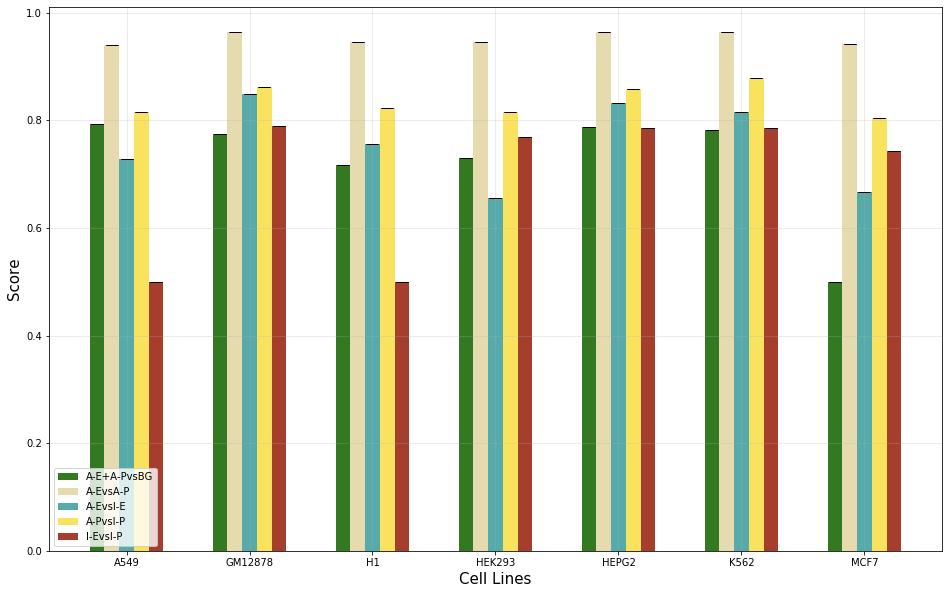
\includegraphics[width=\textwidth]{images/results_plots/single_tasks/unbalanced_new_auroc.png}
        \caption{auROC}
        \label{fig:auroc_unbalanced_new}
    \end{subfigure}
    \begin{subfigure}[b]{\textwidth}
        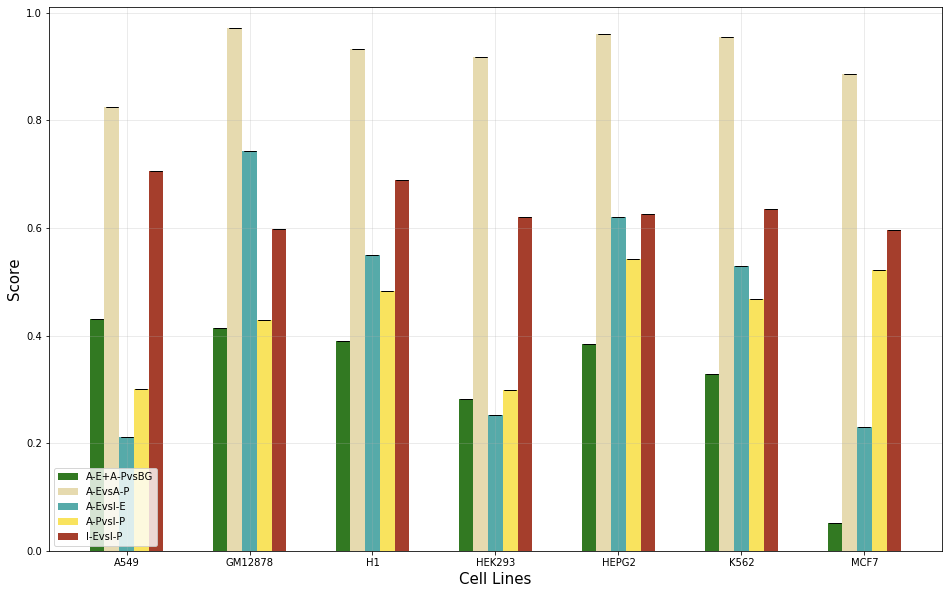
\includegraphics[width=\textwidth]{images/results_plots/single_tasks/unbalanced_new_auprc.png}
        \caption{auPRC}
        \label{fig:auprc_unbalanced_new}
    \end{subfigure}
    \caption{auROC and auPRC for single-task neural network trained using $F_\ell^{\textrm{f1}}$ as features and unbalanced dataset.}\label{fig:unbalanced_new_results}
\end{figure}

\begin{figure}[!htbp]
    \centering
    \begin{subfigure}[b]{\textwidth}
        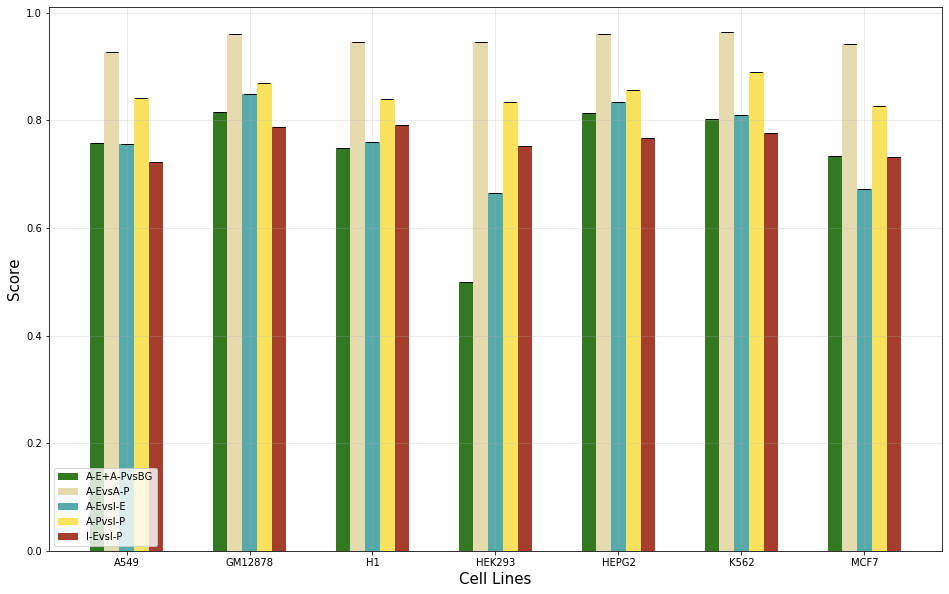
\includegraphics[width=\textwidth]{images/results_plots/single_tasks/balanced_new_auroc.png}
        \caption{auROC}
        \label{fig:auroc_balanced_new}
    \end{subfigure}
    \begin{subfigure}[b]{\textwidth}
        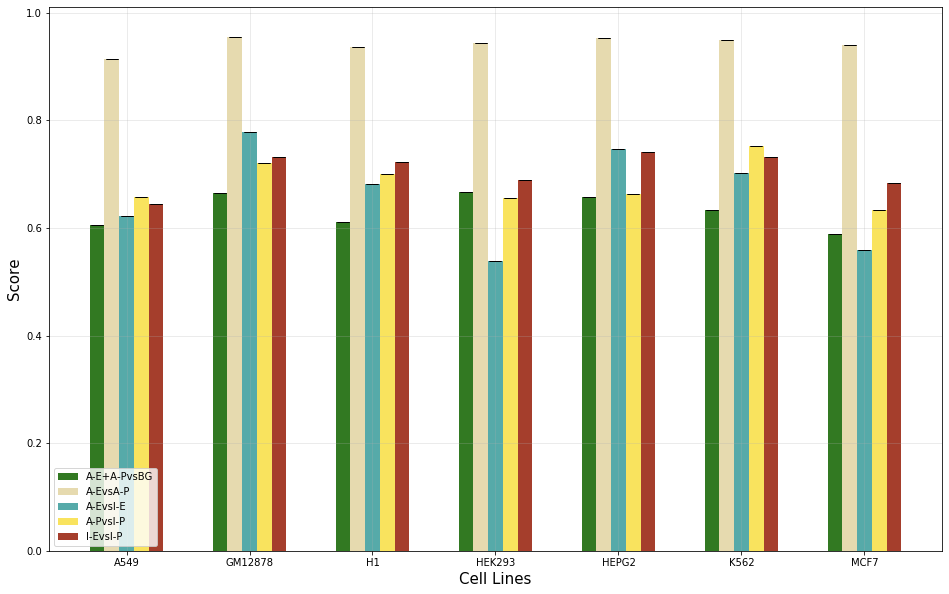
\includegraphics[width=\textwidth]{images/results_plots/single_tasks/balanced_new_auprc.png}
        \caption{auPRC}
        \label{fig:auprc_balanced_new}
    \end{subfigure}
    \caption{auROC and auPRC for single-task neural network trained using $F_\ell^{\textrm{f1}}$ as features and balanced dataset.}\label{fig:balanced_new_results}
\end{figure}

\section{Multi-Task Neural networks results} \label{sec:multi_results}
In this Section we report the results obtained from various experiments performed with the aim to evaluate multi-task neural networks (Section~\ref{sec:MTLsection}) in CRRs classification. We trained the models using different experimental setups explained in Section~\ref{sec:exp_setup_general} and Section~\ref{sec:exp_setup_multitask}. Furthermore, we used both $F_\ell^{\textrm{acc}}$ and $F_\ell^{\textrm{f1}}$ features sets, selected using respectively accuracy and f1-score (Section~\ref{sec:featureselection}).

Initially, the experiments were performed with the first set of features, $F_\ell^{\textrm{acc}}$, and with a fixed number of neurons. In Table~\ref{tab:fixed_neurons_auroc} and Table~\ref{tab:fixed_neurons_auprc} we reported the averages of auROC and auPRC of every holdout with the corresponding standard deviation (STD). In Figure~\ref{fig:fixed_neurons_results} we show the same results visually for easier comparison. Apart from some exceptions, such as I-P vs I-E or A-E vs I-E in HEPG2 and GM12878, looking at Figure~\ref{fig:auprc_fixed_neurons} we can notice that we often have a very low auPRC. 
\begin{figure}[!htbp]
    \centering
    \begin{subfigure}[b]{\textwidth}
        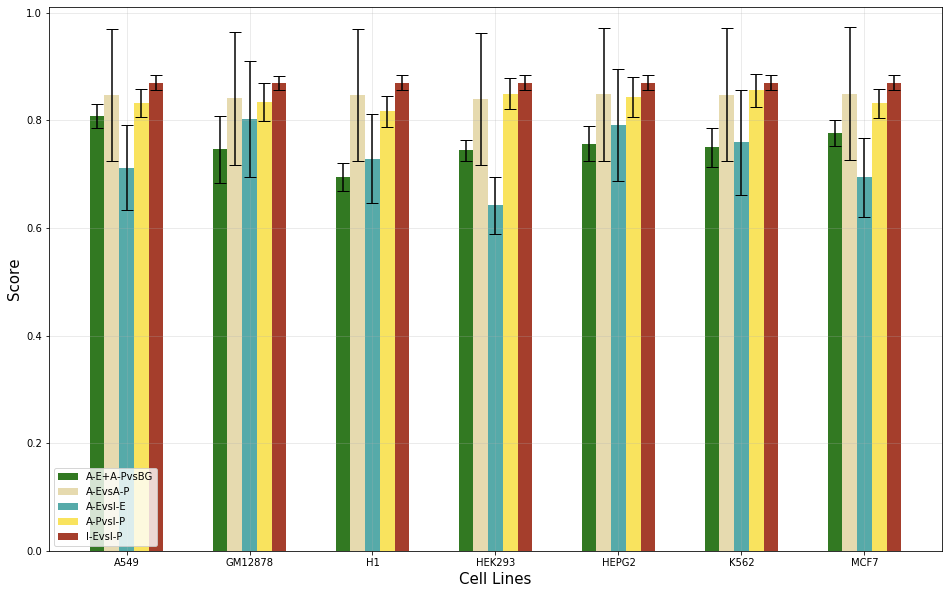
\includegraphics[width=\textwidth]{images/results_plots/fixed_neurons_auroc.png}
        \caption{auROC}
        \label{fig:auroc_fixed_neurons}
    \end{subfigure}
    \begin{subfigure}[b]{\textwidth}
        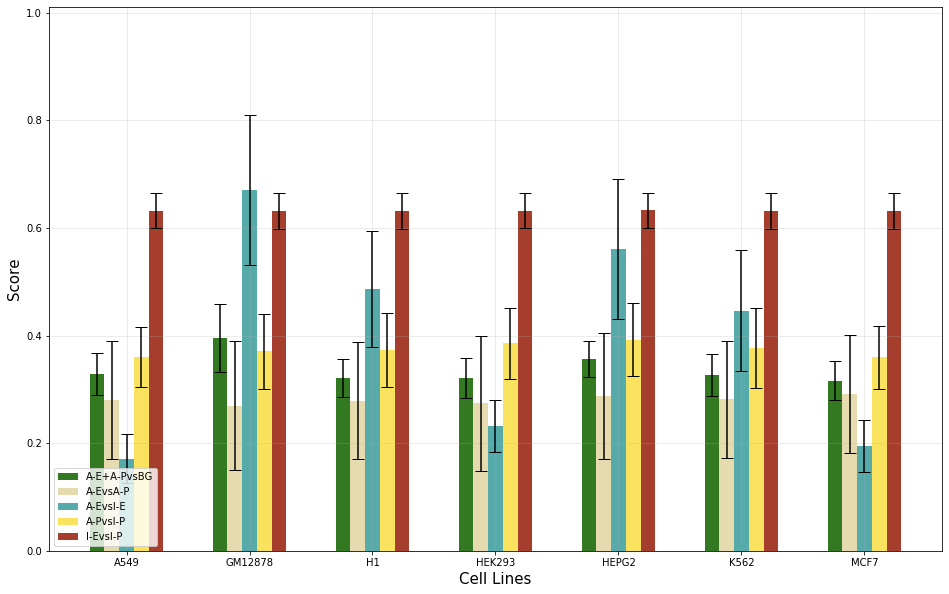
\includegraphics[width=\textwidth]{images/results_plots/fixed_neurons_auprc.png}
        \caption{auPRC}
        \label{fig:auprc_fixed_neurons}
    \end{subfigure}
    \caption{auROC and auPRC for multi-tasks neural network trained using $F_\ell^{\textrm{acc}}$, fixed size of neurons and unbalanced dataset.}
    \label{fig:fixed_neurons_results}
\end{figure}

In order to improve the performance of the models, we tried to balance both training and test set. In Figure~\ref{fig:balanced_results} we reported the bar plots for average auROC (Figure~\ref{fig:auroc_balanced}) and average auPRC (Figure~\ref{fig:auprc_balanced}). Furthermore, in Table~\ref{tab:balanced_auroc} and Table~\ref{tab:balanced_auprc} we summarized the numerical values. We can notice that a performance increase is shown in both auROC and auPRC results. In particular in every cell line $\ell \in L$ and every computational task $p$, excluding A-E vs A-P that remain almost 0.1, we have a noticeable improvement in auPRC.  
%
\begin{figure}[!htbp]
    \centering
    \begin{subfigure}[b]{\textwidth}
        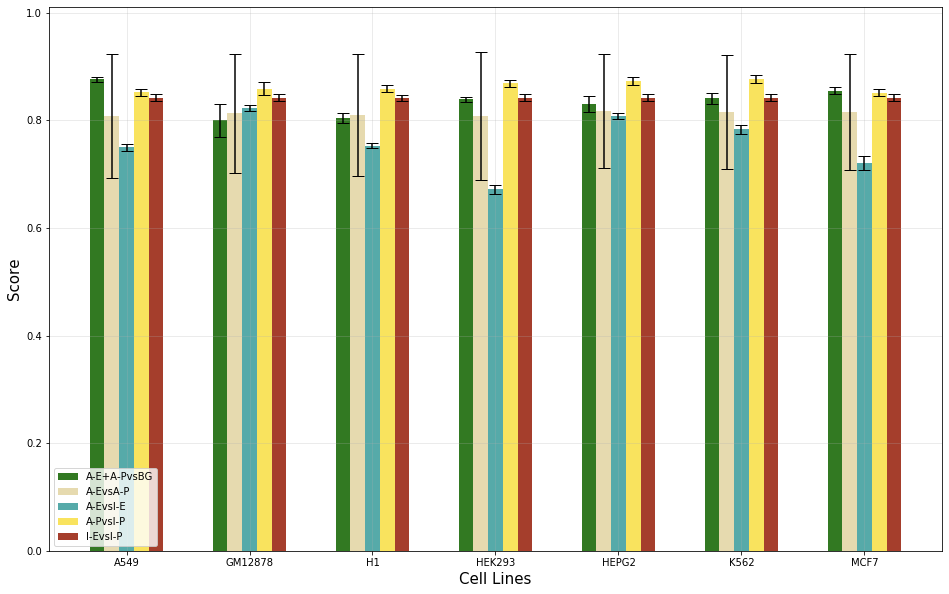
\includegraphics[width=\textwidth]{images/results_plots/balanced_dataset_auroc.png}
        \caption{auROC}
        \label{fig:auroc_balanced}
    \end{subfigure}
    \begin{subfigure}[b]{\textwidth}
        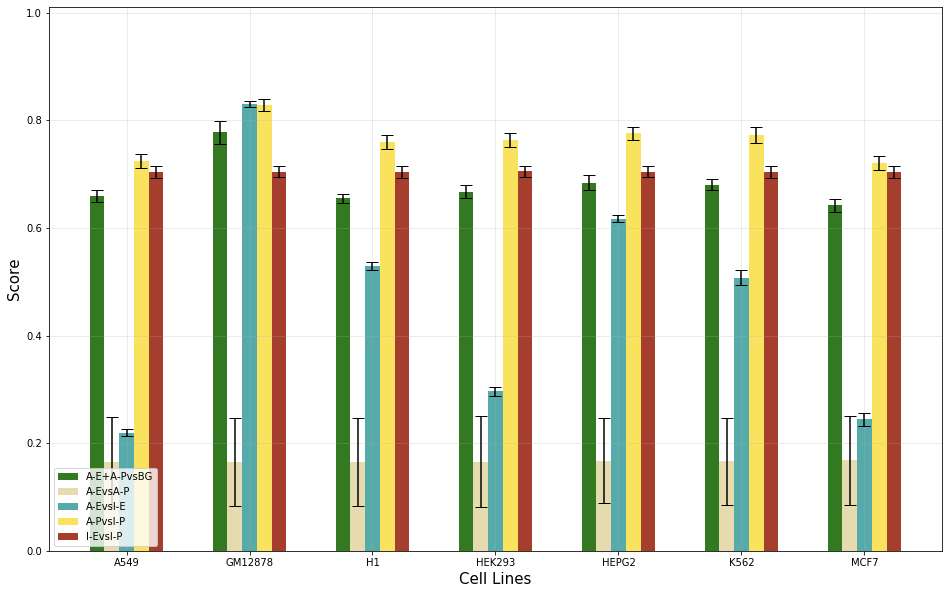
\includegraphics[width=\textwidth]{images/results_plots/balanced_dataset_auprc.png}
        \caption{auPRC}
        \label{fig:auprc_balanced}
    \end{subfigure}
    \caption{auROC and auPRC for multi-tasks neural network trained using $F_\ell^{\textrm{acc}}$, fixed size of neurons and balanced dataset.}
    \label{fig:balanced_results}
\end{figure}

Another experiment performed using $F_\ell^{\textrm{acc}}$ set is the one using a pyramidal architecture. We choose to maintain the dataset balanced due to the good performance highlighted. Overall, compared to the previous fixed neurons configuration, no particular performance improvement emerge using this configuration. The auROC bar plot in Figure~\ref{fig:auroc_pyramydal} shows a slight improvement compared to Figure~\ref{fig:auroc_balanced}. Looking at auPRC values we can notice that there are clear improvements for some tasks, such as A-E vs I-E in MCF7, but a huge decrease for some cell lines (i.e., A549, H1). The results obtained are reported in Figure~\ref{fig:pyramydal_results} and the values summarized in Table~\ref{tab:pyramidal_auroc} and Table~\ref{tab:pyramidal_auprc} in Appendix~\ref{appendix:results_tables}. The standard deviation in both auROC and auPRC has decreased significantly.  
%%
\begin{figure}[!htbp]
    \centering
    \begin{subfigure}[b]{\textwidth}
        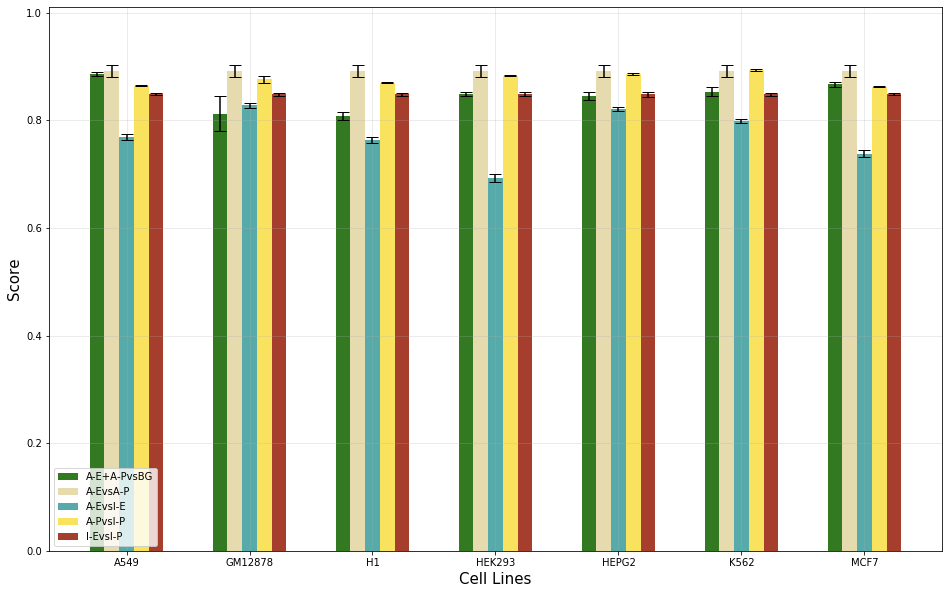
\includegraphics[width=\textwidth]{images/results_plots/pyramydal_auroc.png}
        \caption{auROC}
        \label{fig:auroc_pyramydal}
    \end{subfigure}
    \begin{subfigure}[b]{\textwidth}
        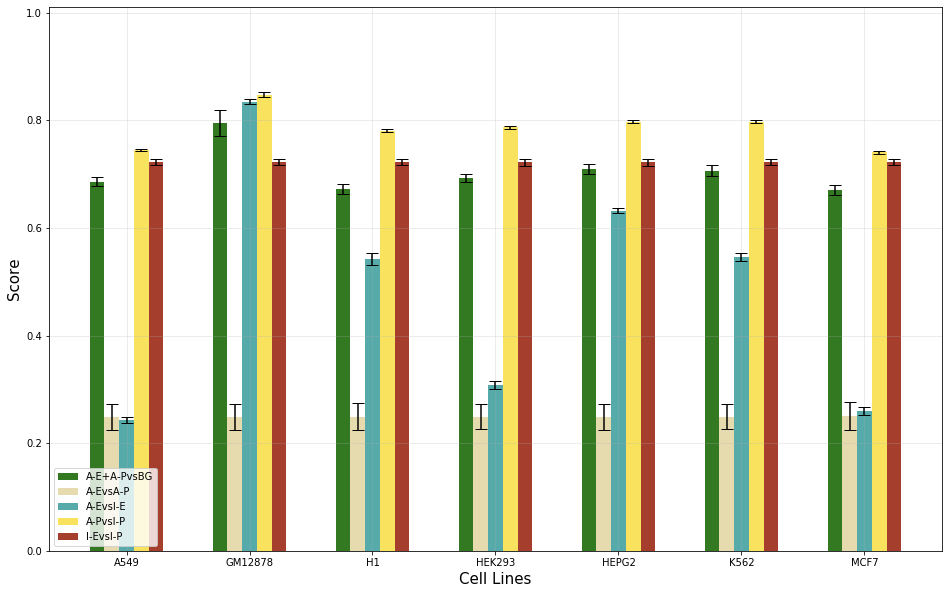
\includegraphics[width=\textwidth]{images/results_plots/pyramydal_auprc.png}
        \caption{auPRC}
        \label{fig:auprc_pyramydal}
    \end{subfigure}
    \caption{auROC and auPRC for multi-tasks neural network trained using $F_\ell^{\textrm{acc}}$, pyramidal structure and balanced dataset.}\label{fig:pyramydal_results}
\end{figure}
%%

In order to test whether the number of tasks influences the performance of the model, we tried to reduce it from seven to four. The idea is that with many tasks could be harder for the model to share knowledge. For those reasons for the last experiment performed on the first set of features, we reduced the set of cell lines $L$ to GM12878, A549, HEPG2 and K562. In Figure~\ref{fig:4celllines_results} we report the average auROC and auPRC obtained, the values are summarized in Table~\ref{tab:4celllines_auprc} and Table~\ref{tab:4celllines_auroc} of Appendix~\ref{appendix:results_tables}. The results show a significant improvement. The average auROC (Figure~\ref{fig:auroc_4celllines}) is greater than 0.8 for every task and every cell lines, sometimes even higher than 0.95. For auPRC bar plot instead, we can see an improvement in many tasks compared to the previous experiments.
%%
\begin{figure}[!htbp]
    \centering
    \begin{subfigure}[b]{\textwidth}
        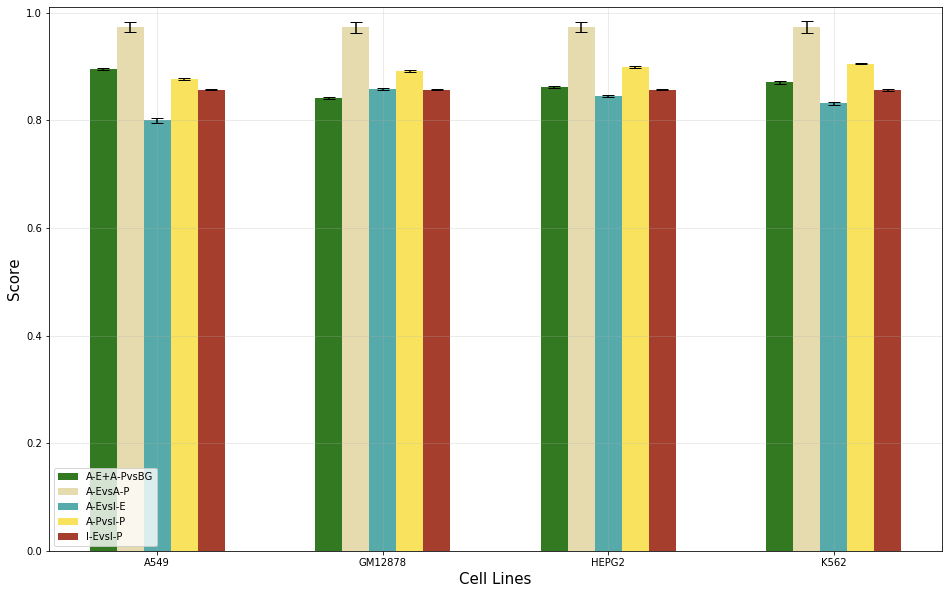
\includegraphics[width=\textwidth]{images/results_plots/4celllines_auroc.png}
        \caption{auROC}
        \label{fig:auroc_4celllines}
    \end{subfigure}
    \begin{subfigure}[b]{\textwidth}
        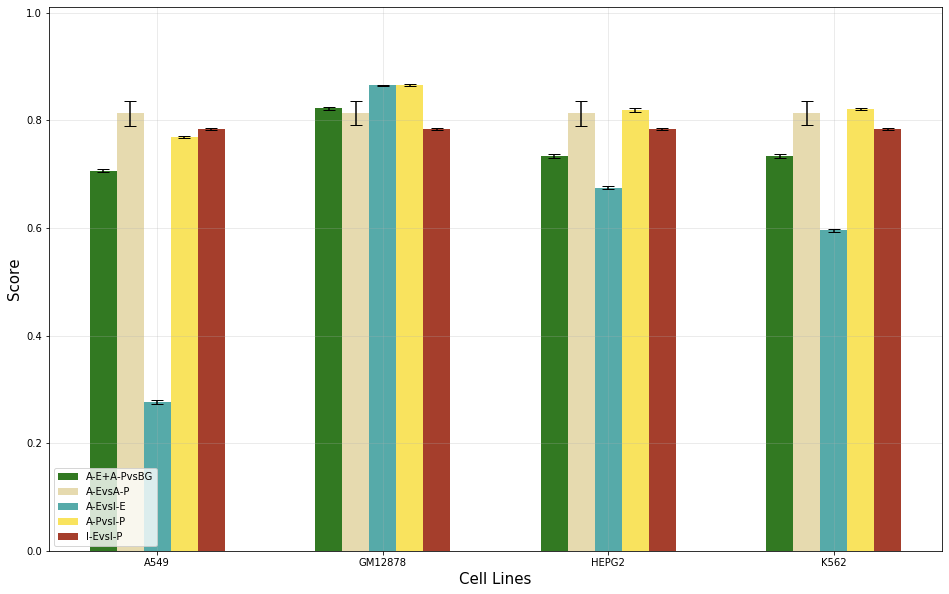
\includegraphics[width=\textwidth]{images/results_plots/4celllines_auprc.png}
        \caption{auPRC}
        \label{fig:auprc_4celllines}
    \end{subfigure}
    \caption{auROC and auPRC for multi-tasks neural network trained using $F_\ell^{\textrm{acc}}$, reduced number of tasks and balanced dataset.}
    \label{fig:4celllines_results}
\end{figure}

Regarding the second set of features $|F_\ell^{\textrm{f1}}|$, chosen using f1-score as evaluating metric, we performed two experiments. The former with neural network pyramidal structure and unbalanced training and test sets, the latter using the same sets of reduced tasks used in the previous experiment (GM12878, A549, HEPG2 and K562) with the balanced dataset. 
\begin{figure}[!htbp]
    \centering
    \begin{subfigure}[b]{\textwidth}
        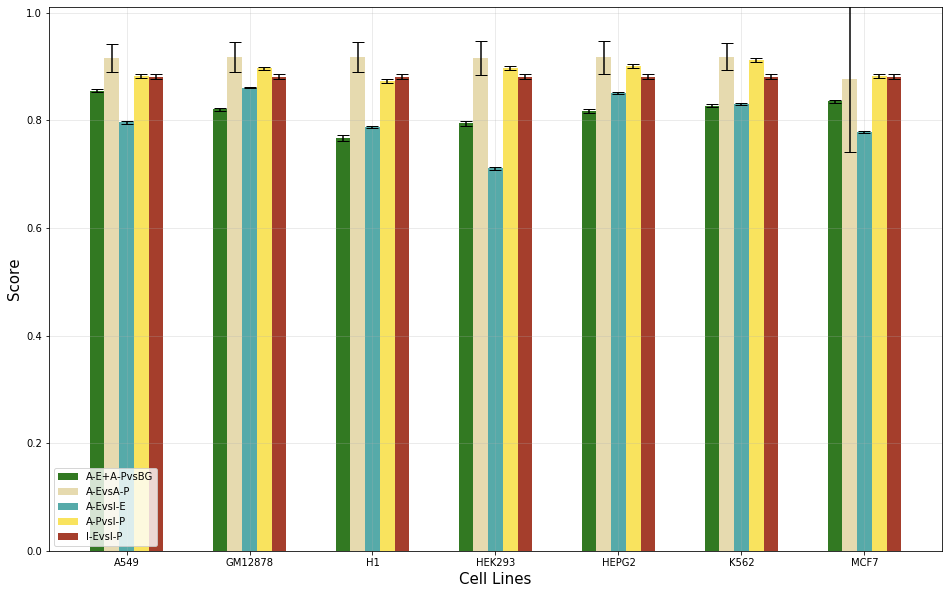
\includegraphics[width=\textwidth]{images/results_plots/new_features_auroc.png}
        \caption{auROC}
        \label{fig:auroc_newfeatures}
    \end{subfigure}
    \begin{subfigure}[b]{\textwidth}
        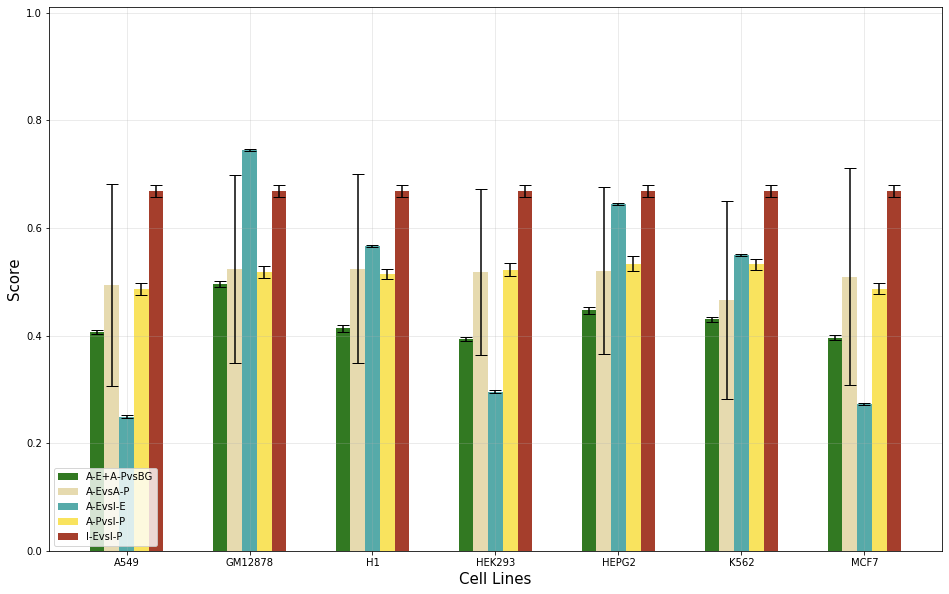
\includegraphics[width=\textwidth]{images/results_plots/new_features_auprc.png}
        \caption{auPRC}
        \label{fig:auprc_newfeatures}
    \end{subfigure}
    \caption{auROC and auPRC for multi-tasks neural network trained using $F_\ell^{\textrm{f1}}$, pyramidal structure and unbalanced dataset.}\label{fig:newfeatures_results}
\end{figure}
%%
\begin{figure}[!htbp]
    \centering
    \begin{subfigure}[b]{\textwidth}
        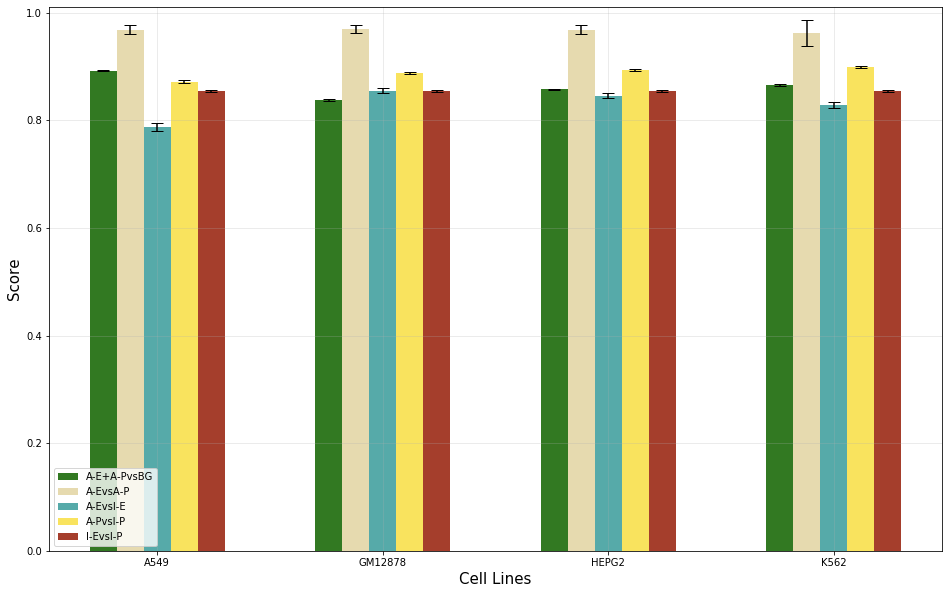
\includegraphics[width=\textwidth]{images/results_plots/4celllines_new_auroc.png}
        \caption{auROC}
        \label{fig:auroc_new_4celllines}
    \end{subfigure}
    \begin{subfigure}[b]{\textwidth}
        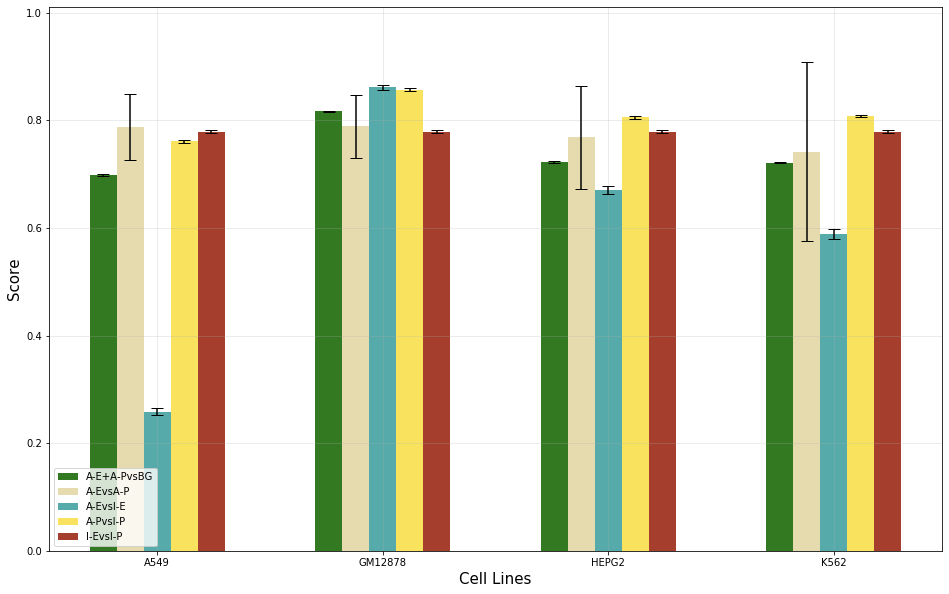
\includegraphics[width=\textwidth]{images/results_plots/4celllines_new_auprc.png}
        \caption{auPRC}
        \label{fig:auprc_new_4celllines}
    \end{subfigure}
   \caption{auROC and auPRC for multi-tasks neural network trained using $F_\ell^{\textrm{f1}}$, reduced number of tasks and balanced dataset.}\label{fig:new_4celllines_results}
\end{figure}

In Figure~\ref{fig:newfeatures_results} and Figure~\ref{fig:new_4celllines_results} we reported the results obtained respectively with the first and second experiments. The values of auROC and auPRC are summarized in Table~\ref{tab:newfeatures_auprc} and Table~\ref{tab:newfeatures_auroc} for the first experiments and in Table~\ref{tab:new_4celllines_auroc} and Table~\ref{tab:new_4celllines__auprc} for the second. 
In both experiments no particular differences emerge comparing with the previous experiments performed (Figure~\ref{fig:fixed_neurons_results} and Figure~\ref{fig:4celllines_results}).

\section{Single-Task and Multi-Task Neural Networks Comparison}
\label{sec:results_discussion}
In this Section we compare and discuss the results obtained by single-task and multi-tasks neural network experiments. As already seen, the best results are obtained with the balanced dataset in both single-task and multi-tasks. Therefore, seems that there is a minor difference in performance using $F_\ell^{\textrm{acc}}$ or $F_\ell^{\textrm{f1}}$. In some experiments using the first features set give slightly better results. 

The most obvious difference comparing the results obtained by the two models is that single-task neural networks are better in distinguishing active enhancers from active promoters. This behaviour is evident comparing, for instance, results obtained using single-tasks neural network and the multi-tasks with pyramidal structure using the unbalanced dataset with the first set of features (Figure~\ref{fig:unbalanced_old_results} and Figure~\ref{fig:pyramydal_results}). The same results are obtained in almost every configuration. Note that, A-E vs A-P is the computational task with less data. A possible explanation of this phenomenon is the complexity of multi-task neural networks architecture that, in some cases, could contains many parameters. With small dataset, this complexity could lead to model over-fitting. 

Overall, based on our experiments, we can say that multi-tasks neural networks are better in distinguishing active enhancers and active promoters (A-E+A-P) from everything else (BG), active promoters from inactive promoters and inactive enhancers from inactive promoters. This behaviour is evident in almost every experimental setup. For instance, despite the fixed size neurons configurations is resulted in the worst for multi-tasks neural networks, comparing its results with those of single-task neural network we can notice that they are often comparable or even slightly better.

We did not get promising results using the multi-tasks neural network with fixed neurons setup. In fact, comparing the results reported in Figure~\ref{fig:fixed_neurons_results} with, for instance, the results of single-task neural network reported in Figure~\ref{fig:unbalanced_old_results} we can notice that they are very similar.

The most promising results for multi-task neural networks are obtained using a pyramidal structure. In fact, with balanced training and test sets and using the accuracy selected features $F_\ell^{\textrm{acc}}$, the results obtained by this model overcome the one obtained by the single task neural network in many computational tasks. Comparing Figure~\ref{fig:balanced_old_results} and Figure~\ref{fig:pyramydal_results} we can notice that, apart from active enhancers versus active promoters and active enhancers vs inactive enhancers, the pyramidal multi-tasks approach always give better results than the single-task counterpart. This is true both for average auROC (Figure~\ref{fig:auroc_balanced_old} and Figure~\ref{fig:auroc_pyramydal}) and average auPRC (Figure~\ref{fig:auprc_balanced_old} and Figure~\ref{fig:auprc_pyramydal}). In Table~\ref{tab:pyramidal_auroc} and Table~\ref{tab:pyramidal_auprc} of Appendix~\ref{appendix:results_tables} the results of the computational task that obtained higher results respect their single-task counterpart are highlighted in bold. We obtained a similar but less evident results using the f1-score selected features set. 

Regarding the multi-tasks experiments using a reduced set of tasks, we obtained very promising results. In both features setups we obtained very high auROC and auPRC values. In average auROC, reported in Figure~\ref{fig:auroc_4celllines} and Figure~\ref{fig:auroc_new_4celllines}, the results always exceed 0.8. Regarding average auPRC instead, we obtained very good results. These results, compared to the best single tasks model results, are higher for most computational tasks. Despite reducing the tasks has greatly improved the performance, probably because is easier for the model learn a common representation, the multi-tasks neural networks fail to overcome single-task neural networks in distinguish active enhancers and active promoters. 


In Figure~\ref{fig:4celllines_comparison} we put side-by-side the bar plots of the two considered models. We used $F_\ell^{\textrm{acc}}$ as set of feature, the reduced set of cell lines and a balanced dataset setting. Every computational task is represented by a colour (green, grey, blue, yellow and red), darker and lighter respectively for single-task and the multi-tasks models. 
To compare the two results, we applied a popular non-parametric statistical hypothesis test called Wilcoxon singed-rank test \cite{Wilcoxon1945IndividualCB}. Fixed a task, the test is performed concatenating the auROC and auPRC for every cell lines obtaining two vectors, one for single-tasks results and one for multi-tasks results. These two vector are the input of Wilcoxon signed-rank test. We reported the results of this test in Table~\ref{tab:wilcoxon} where the $p$-values under a threshold of 0.01 are reported in bold. We can notice that in this experiment multi-task model is better in distinguishing active promoters from inactive promoters, inactive enhancers from inactive promoters and active enhancers and active promoters from everything else. 

\begin{figure}[!htbp]
    \centering
    \begin{subfigure}[b]{\textwidth}
        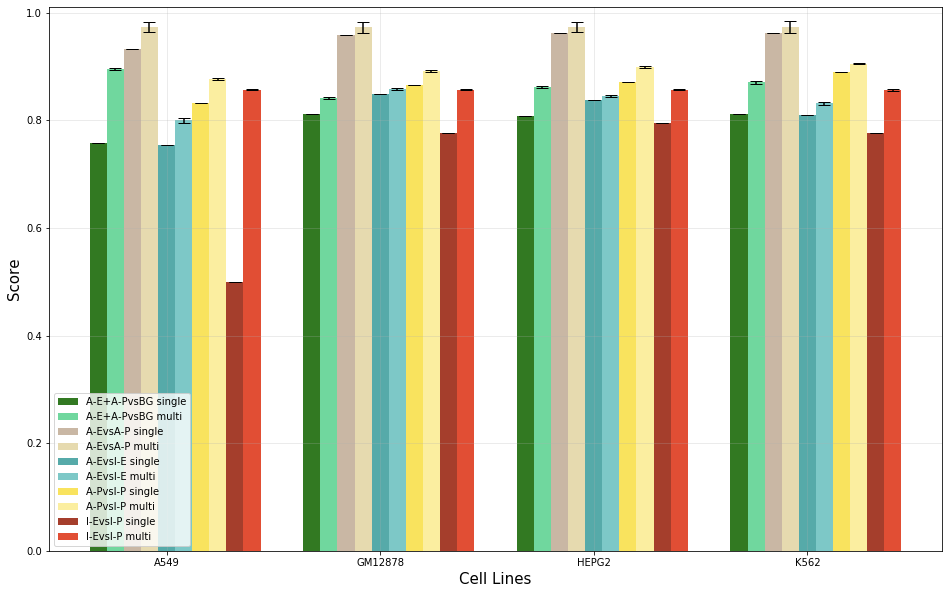
\includegraphics[width=\textwidth]{images/results_plots/auroc_4celllines_comparison.png}
        \caption{auROC}
        \label{fig:auroc_new_4celllines_comparison}
    \end{subfigure}
    \begin{subfigure}[b]{\textwidth}
        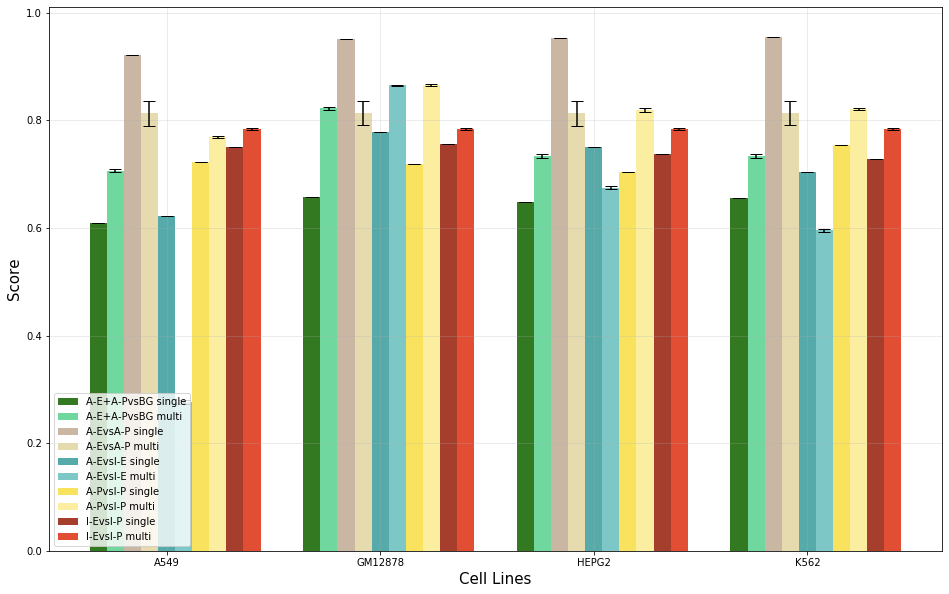
\includegraphics[width=\textwidth]{images/results_plots/auprc_4celllines_comparison.png}
        \caption{auPRC}
        \label{fig:auprc_new_4celllines_comparison}
    \end{subfigure}
   \caption{auROC and auPRC comparison between the two considered models, single-task and multi-tasks. We used $F_\ell^{\textrm{acc}}$, reduced number of tasks and balanced dataset.} 
   \label{fig:4celllines_comparison}
\end{figure}

\begin{table}[!htbp]
\centering
\begin{tabular}[t]{lcccl}
\toprule
Computational Task & Win & Tie & Loss & $p$-value\\
\midrule
A-E+A-PvsBG & 8 & 0 & 0 & \textbf{0.0078125} \\
A-EvsA-P & 4 & 0 & 4 & 0.3125 \\
A-EvsI-E & 5 & 0 & 3 & 0.84375 \\
A-PvsI-P & 8 & 0 & 0 & \textbf{0.0078125} \\
I-EvsI-P & 8 & 0 & 0 & \textbf{0.0078125} \\
\bottomrule
\end{tabular}
\caption{auROC and auPRC Wilcoxon signed-rank test for the two considered models, single-task and multi-tasks. We used $F_\ell^{\textrm{acc}}$, reduced number of tasks and balanced dataset.}
\label{tab:wilcoxon}
\end{table}

\chapter{Conclusion}
Within this work, we tried to understand whether multi-task deep learning methods outperform state-of-the-art models in distinguishing cis-regulatory regions across the genome. 

Our works focused on neural networks MTL. In particular, hard-parameters sharing approaches (Section~\ref{sec:MTLsection}). Classical feed-forward neural networks (single-task neural networks) was chosen as a benchmark (Section~\ref{sec:singletaskNN}). This choice is due to the excellent results in CRRs classification highlighted in previous works. To select the best hyper-parameters configurations of our models, a Gaussian Process has been used (Section~\ref{sec:gaussianprocess}).
To train our models, we gathered epigenetic features and regions labels from ENCODE and FANTOM (Section~\ref{sec:epigenomic_data}). We also introduced feature selection methods to reduce the large number of features, especially in some cell lines (Section~\ref{sec:featureselection}). Using these methods we selected two different reduced features sets. 
Analyzing the performance, after running the experimental setups described in Chapter~\ref{cap:experimental_seup}, we obtained promising results. Note that, the results obtained with both features sets are comparable and does not present significant differences. 

The single-task neural network ability to distinguish cis-regulatory regions is confirmed. In fact, we obtained excellent results in both considered metrics (Section~\ref{sec:methods_metrics}), in particular with the dataset balanced. Furthermore, our experiments highlight the ability of single-task neural networks to distinguish active promoters and active enhancers (Figure~\ref{fig:unbalanced_old_results} and Figure~\ref{fig:balanced_new_results}).

Our experiments using multi-tasks neural networks models gave promising results. In many computational tasks, as described in Section~\ref{sec:multi_results} and Section~\ref{sec:results_discussion}, they obtain better results than single-tasks neural networks.
In general, the proposed models result better in distinguishing: active enhancers and active promoters from everything else, active promoters from inactive promoters and, finally, inactive enhancer from inactive promoters. In addition, our studies have shown that, also with an MTL setting, a pyramidal structure of the network gives better results compared to fixing the size of neurons of every layer. 
Finally, we could notice that reducing the number of tasks (cell lines) involved in the training process improved the performances significantly. 

Although our works give exciting insight about multi-task learning neural networks ability to classify CRRs, there is still much work to be done. In particular, we suggest to try other MTL approaches not considered in this work: for instance, neural networks based, such as soft-parameters sharing, or non-neural models. Besides, some efforts can be dedicated to studying an approach that permits to understand how much the cell lines are related. Probably, training multi-task learning models with highly related tasks lead to better performance. It is also possible that the architecture of the multi-tasks network is too complex for the problem at hand. We could e.g. remove the output branches, reduce the number of hidden layers of each module or both. 

The importance of recognizing regulatory elements across human DNA, due to the serious health implications in misregulation of genes, and the promising results that we obtained in our investigations makes us believe that continuing research in that direction can bring significant results. 


\appendix
\chapter{t-SNE Decomposition} \label{appendix:tsne}
\begin{figure}[h]
\centering
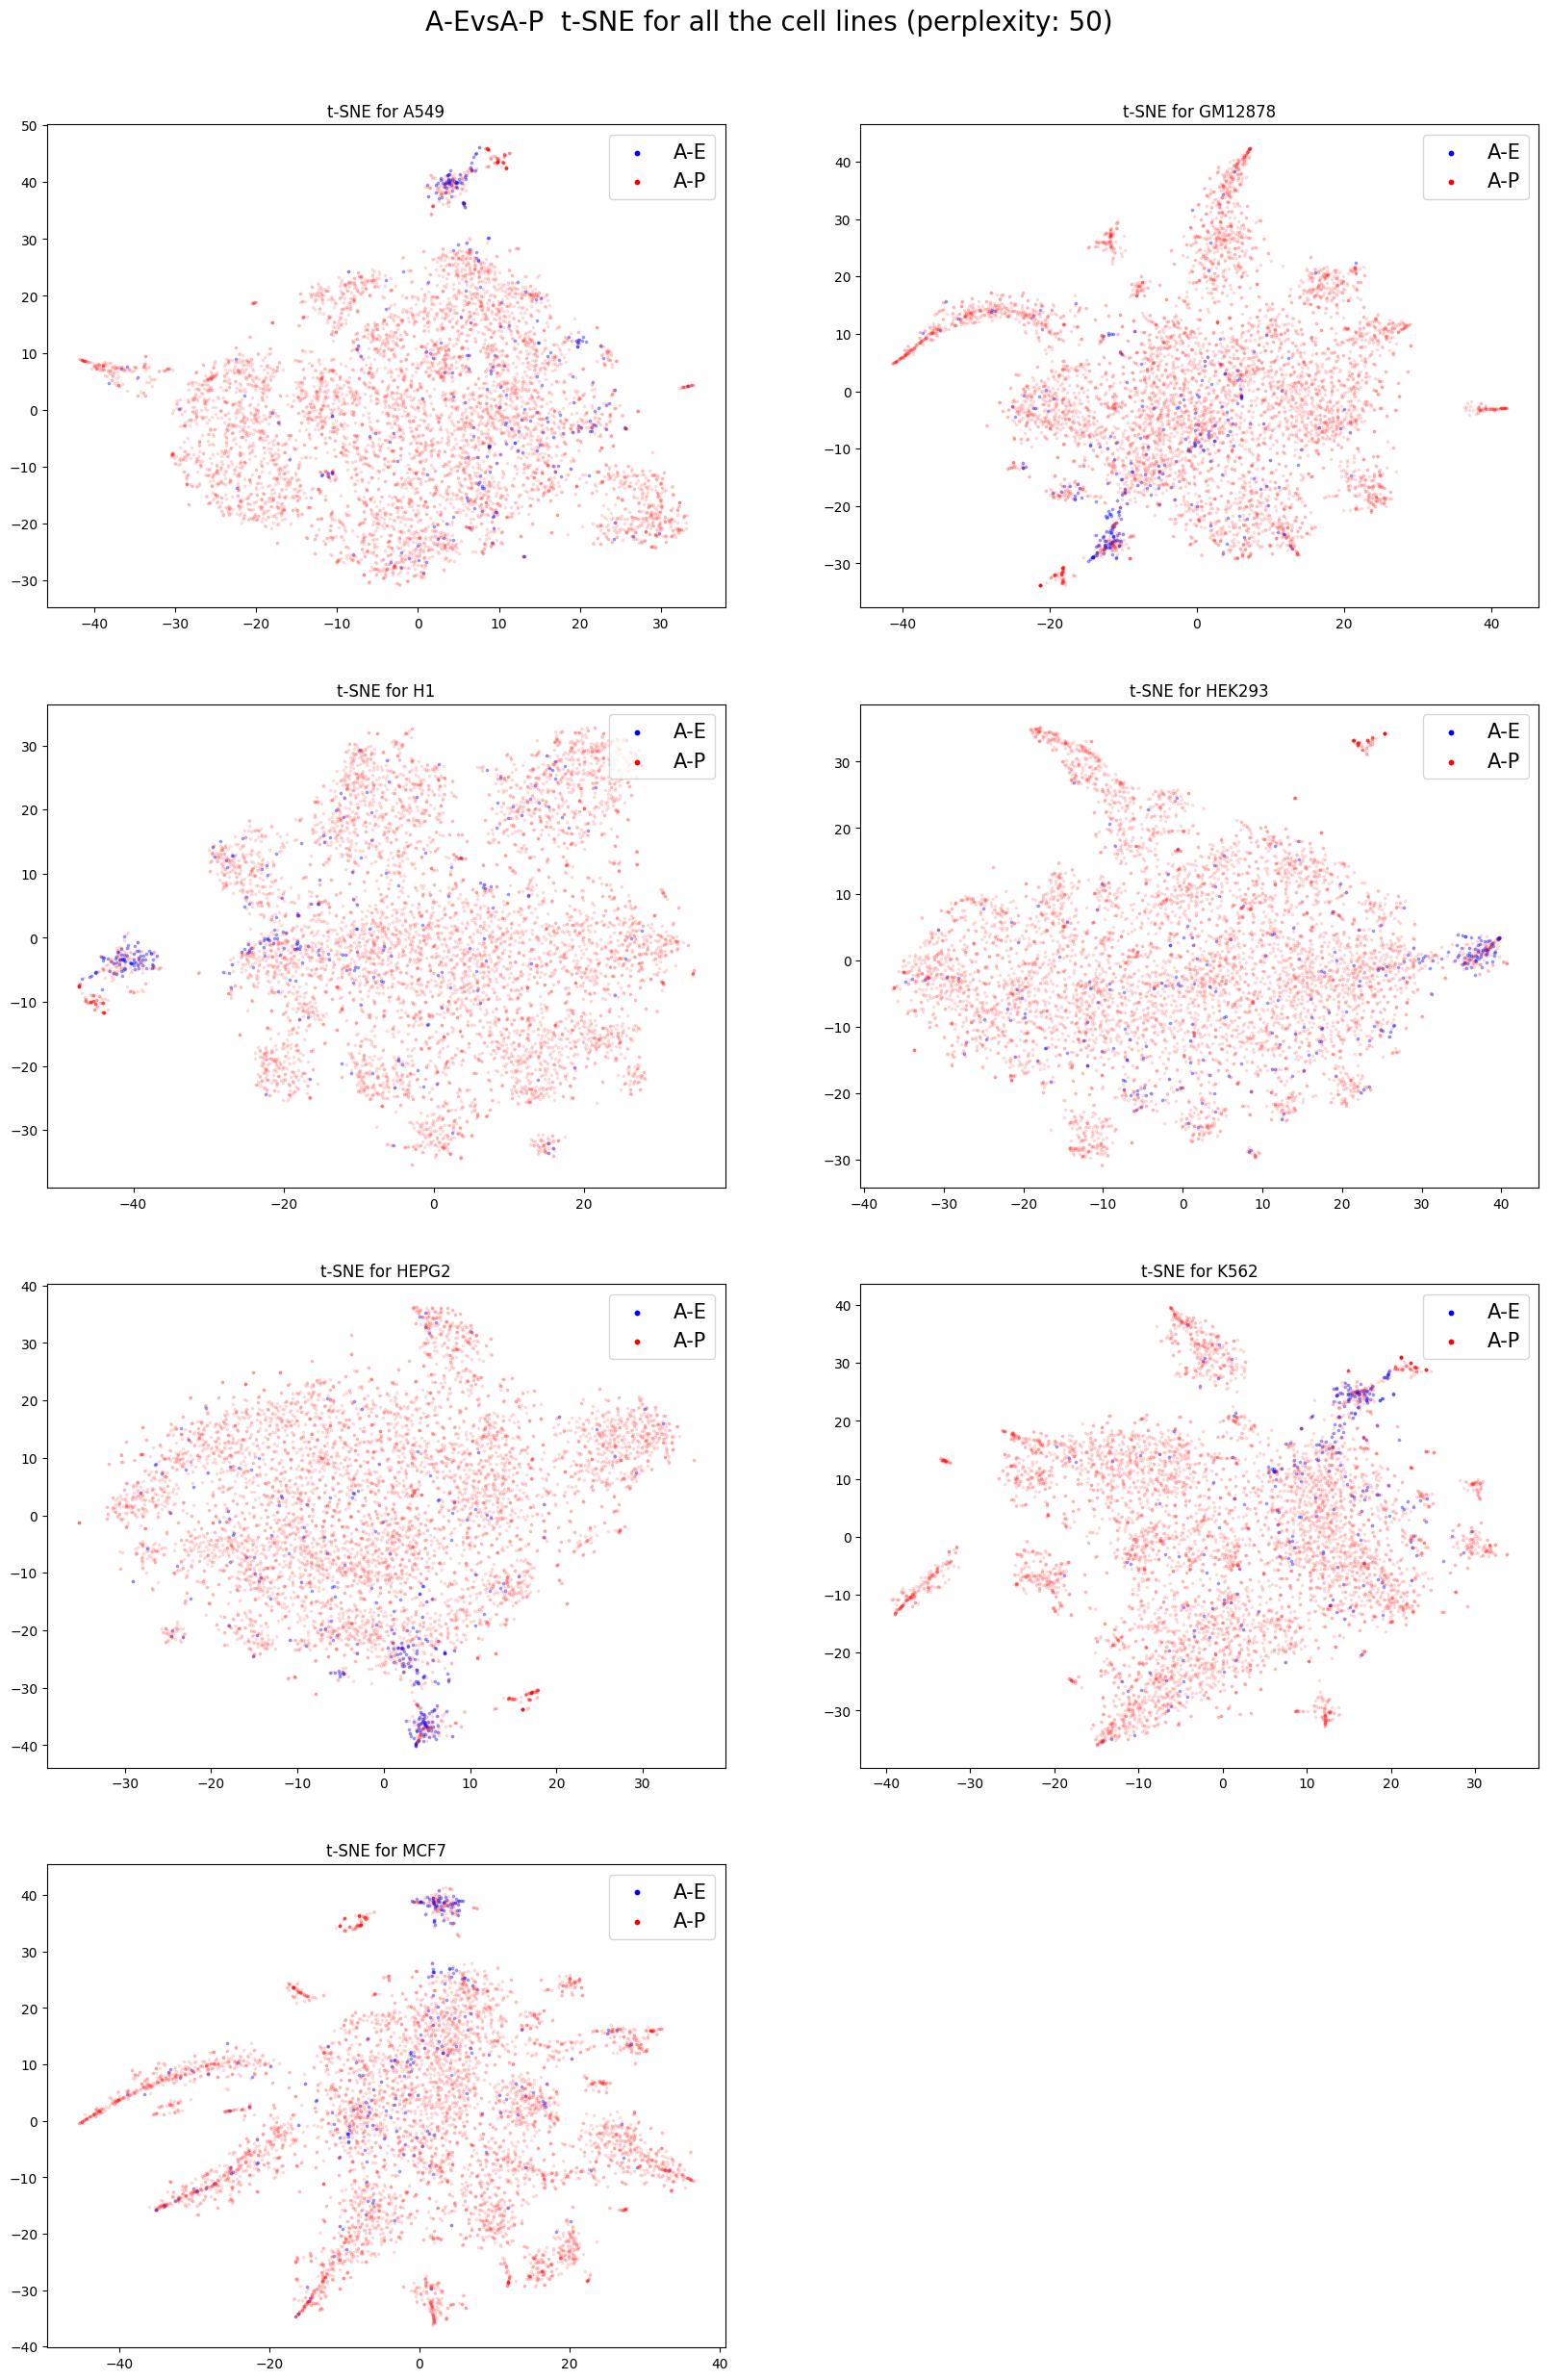
\includegraphics[width=12cm]{images/tsne_decomp_plots/20200410-232525_A-EvsA-P_tsne_plot.png}
\caption{t-SNE for A-E vs A-P}
\label{fig:tsneAEvsAP}
\end{figure}

\begin{figure}[h]
\centering
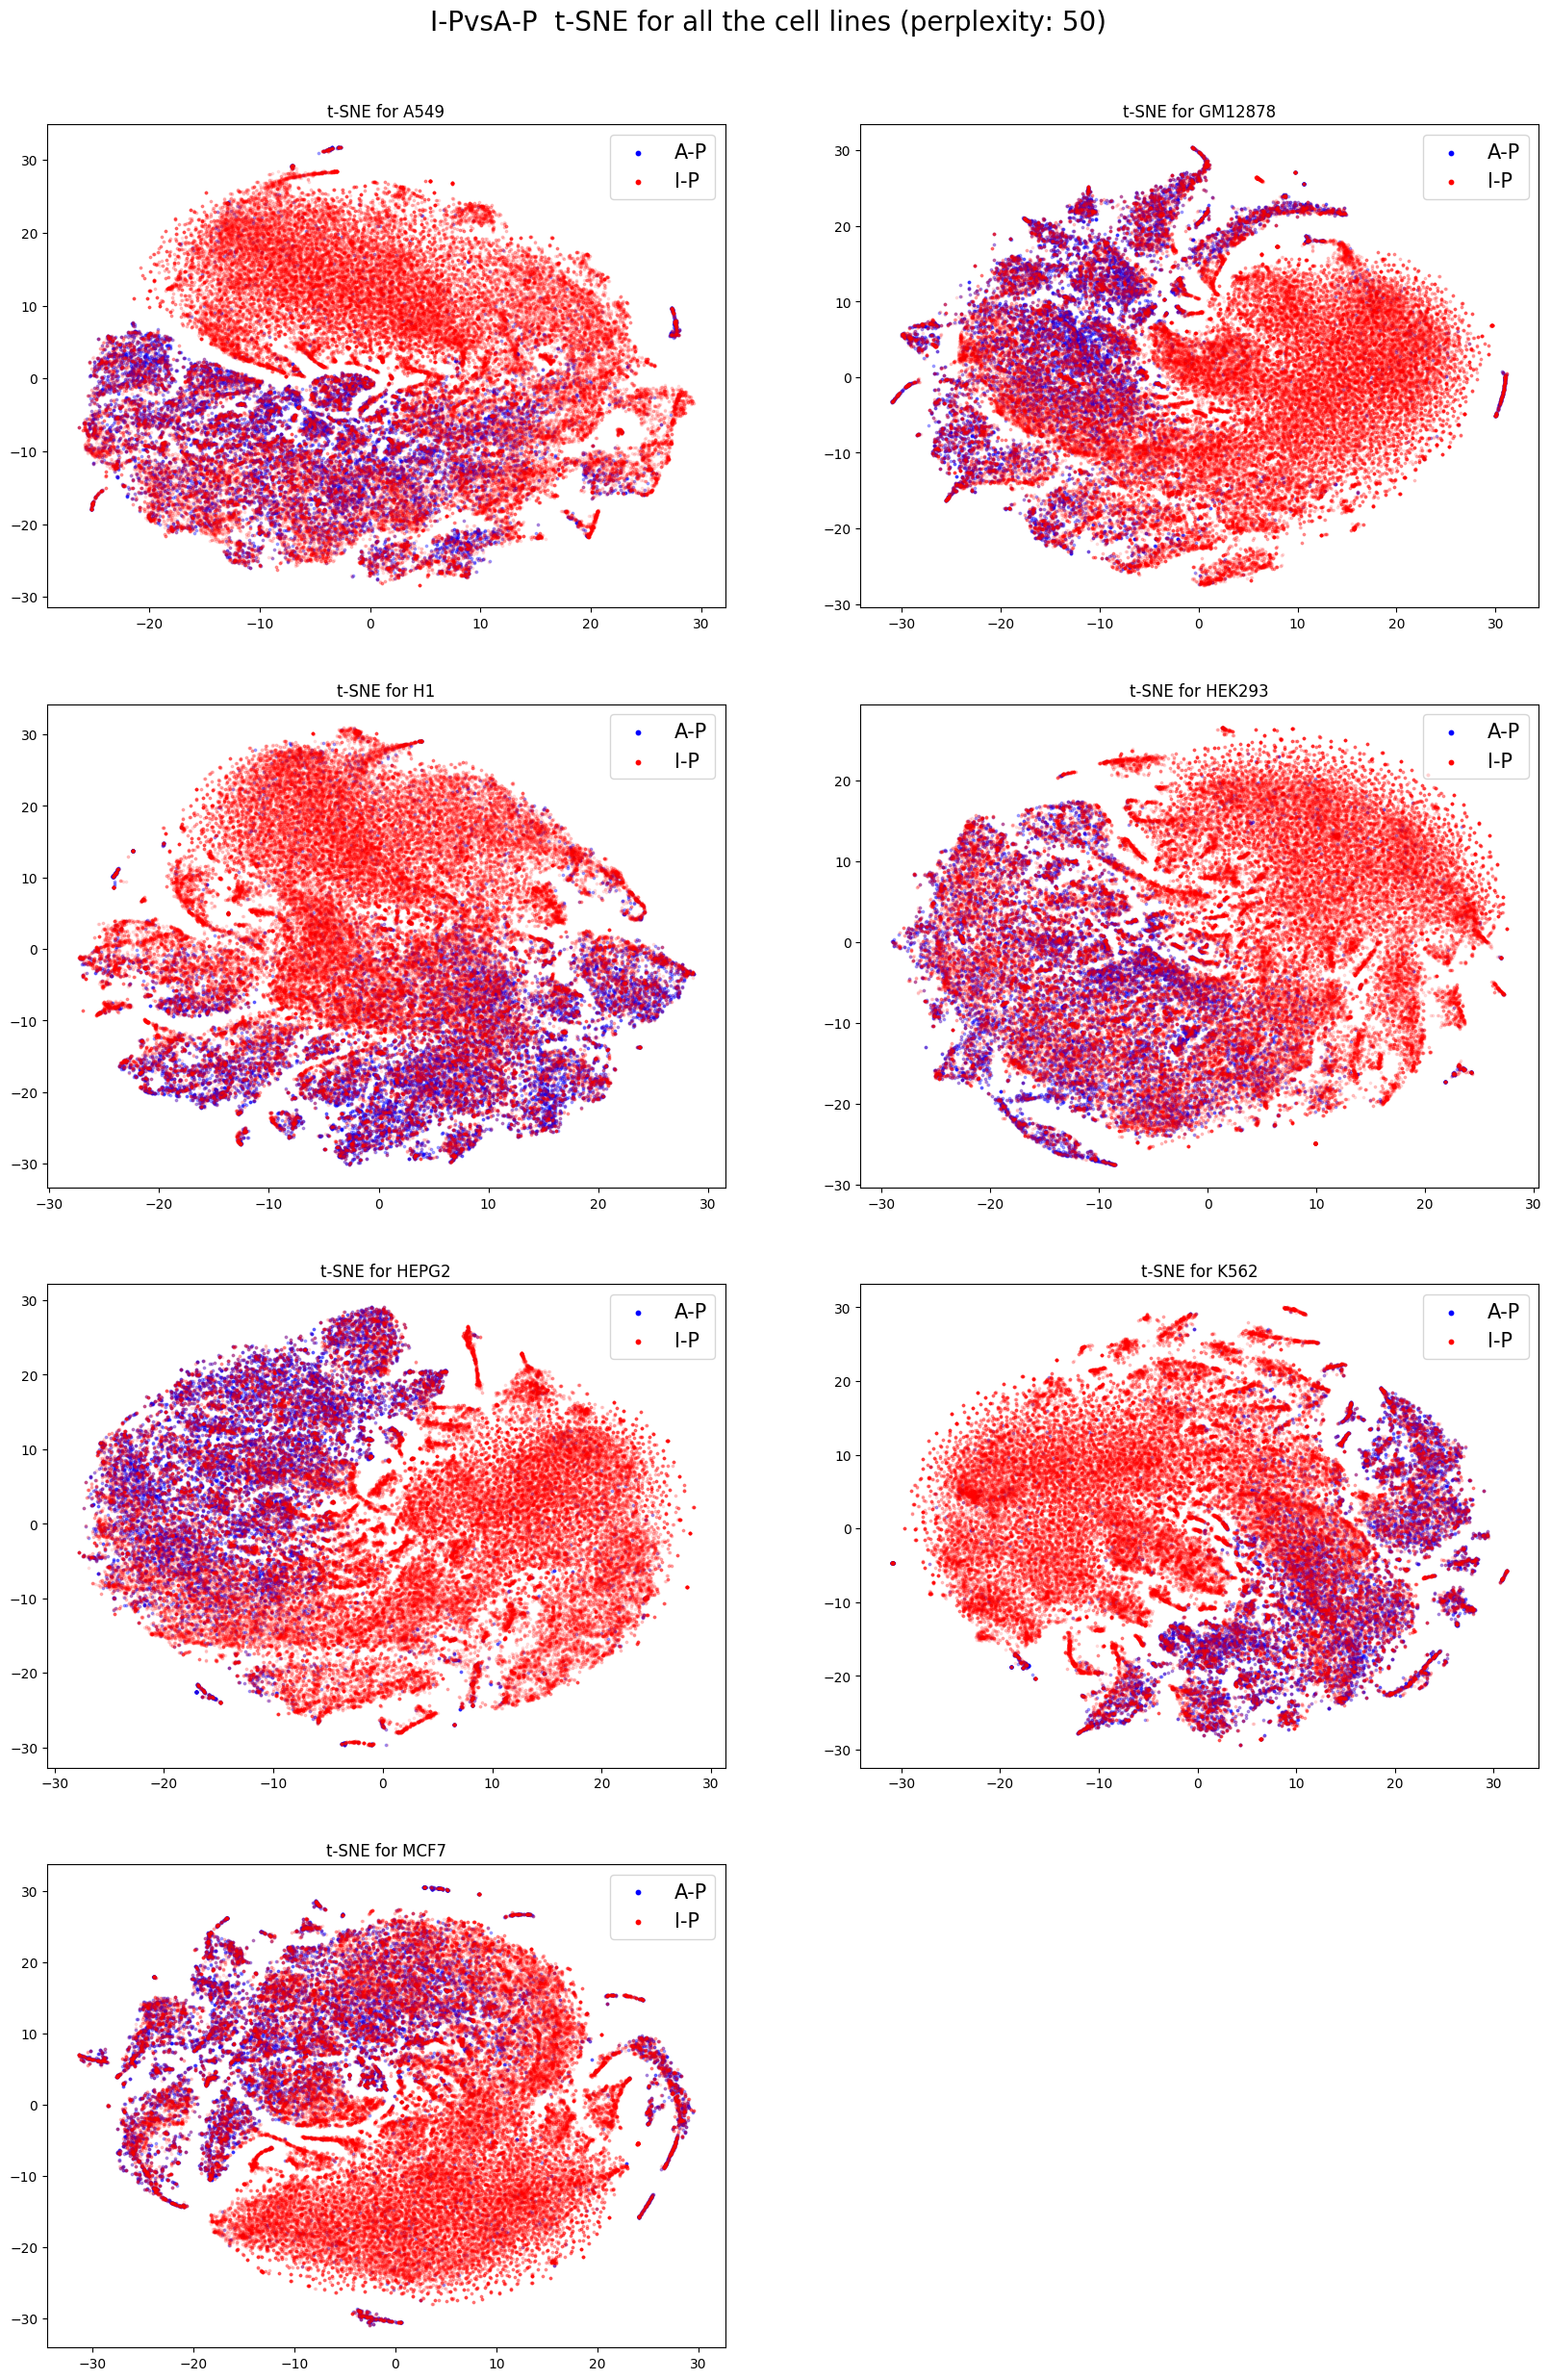
\includegraphics[width=12cm]{images/tsne_decomp_plots/20200410-232531_I-PvsA-P_tsne_plot.png}
\caption{t-SNE for I-P vs A-P}
\label{fig:tsneIPvsAP}
\end{figure}

\begin{figure}[h]
\centering
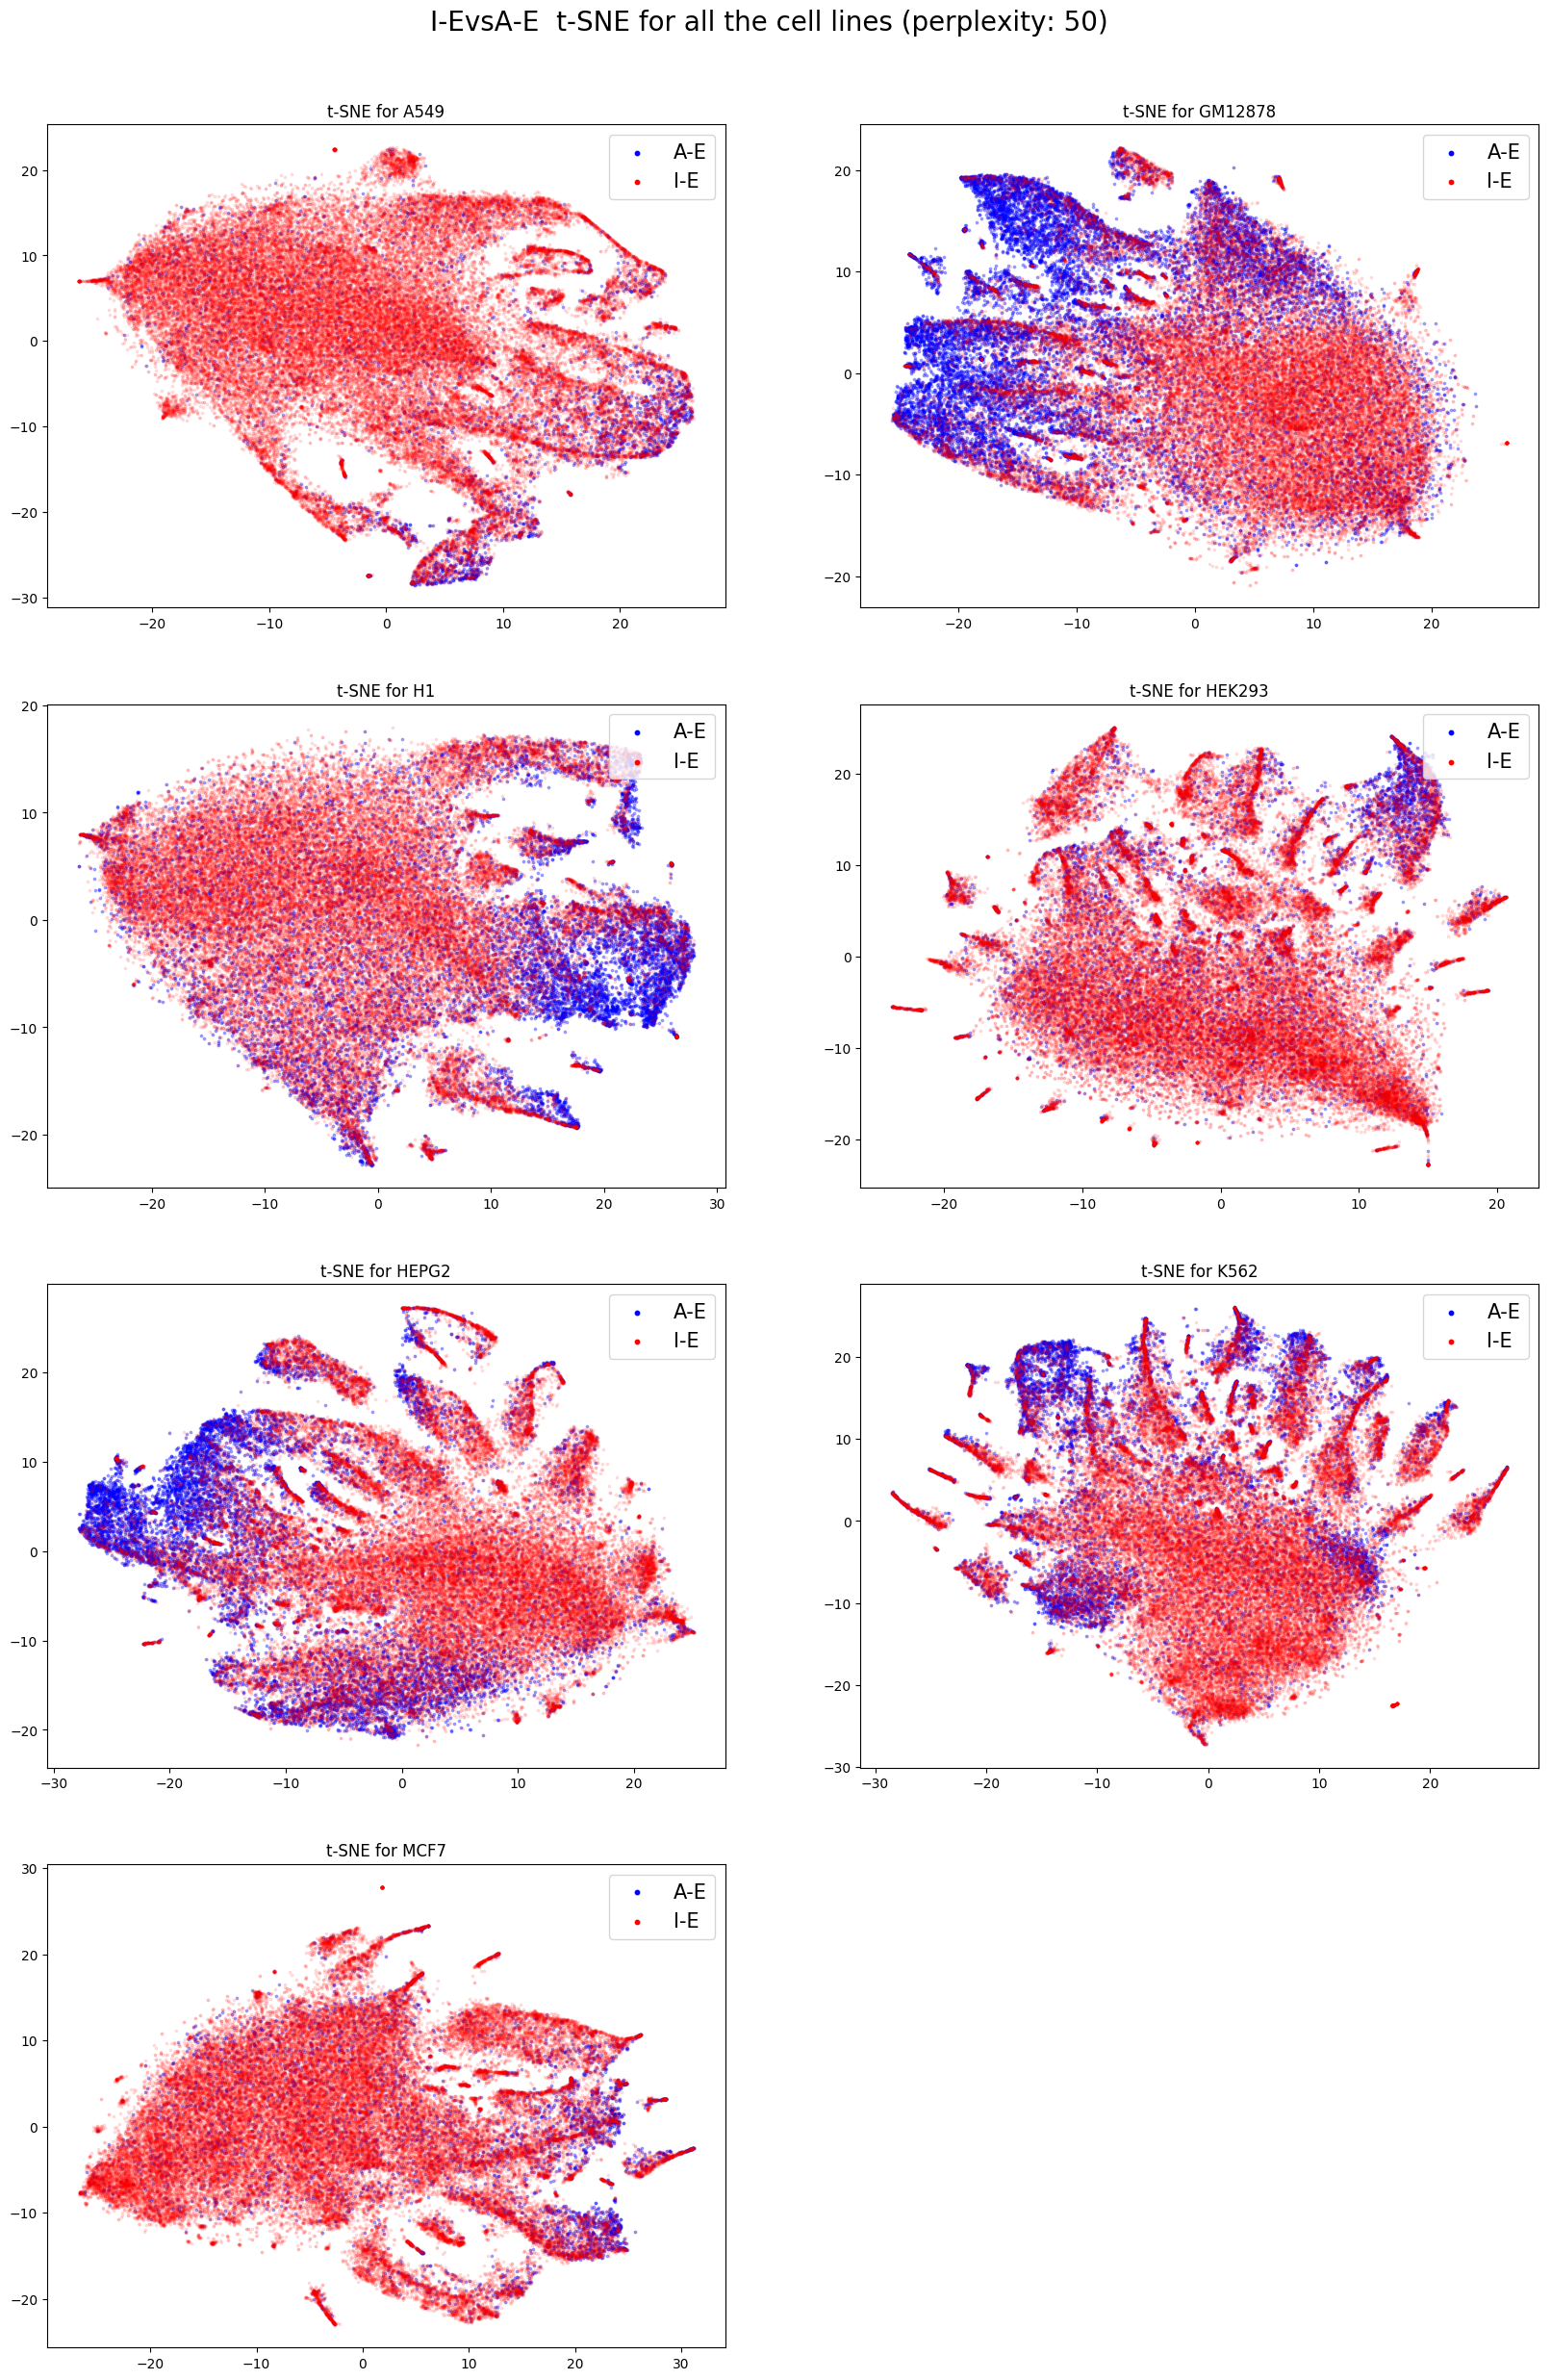
\includegraphics[width=12cm]{images/tsne_decomp_plots/20200410-232543_I-EvsA-E_tsne_plot.png}
\caption{t-SNE for I-E vs A-E}
\label{fig:tsneIEvsAE}
\end{figure}

\begin{figure}[h]
\centering
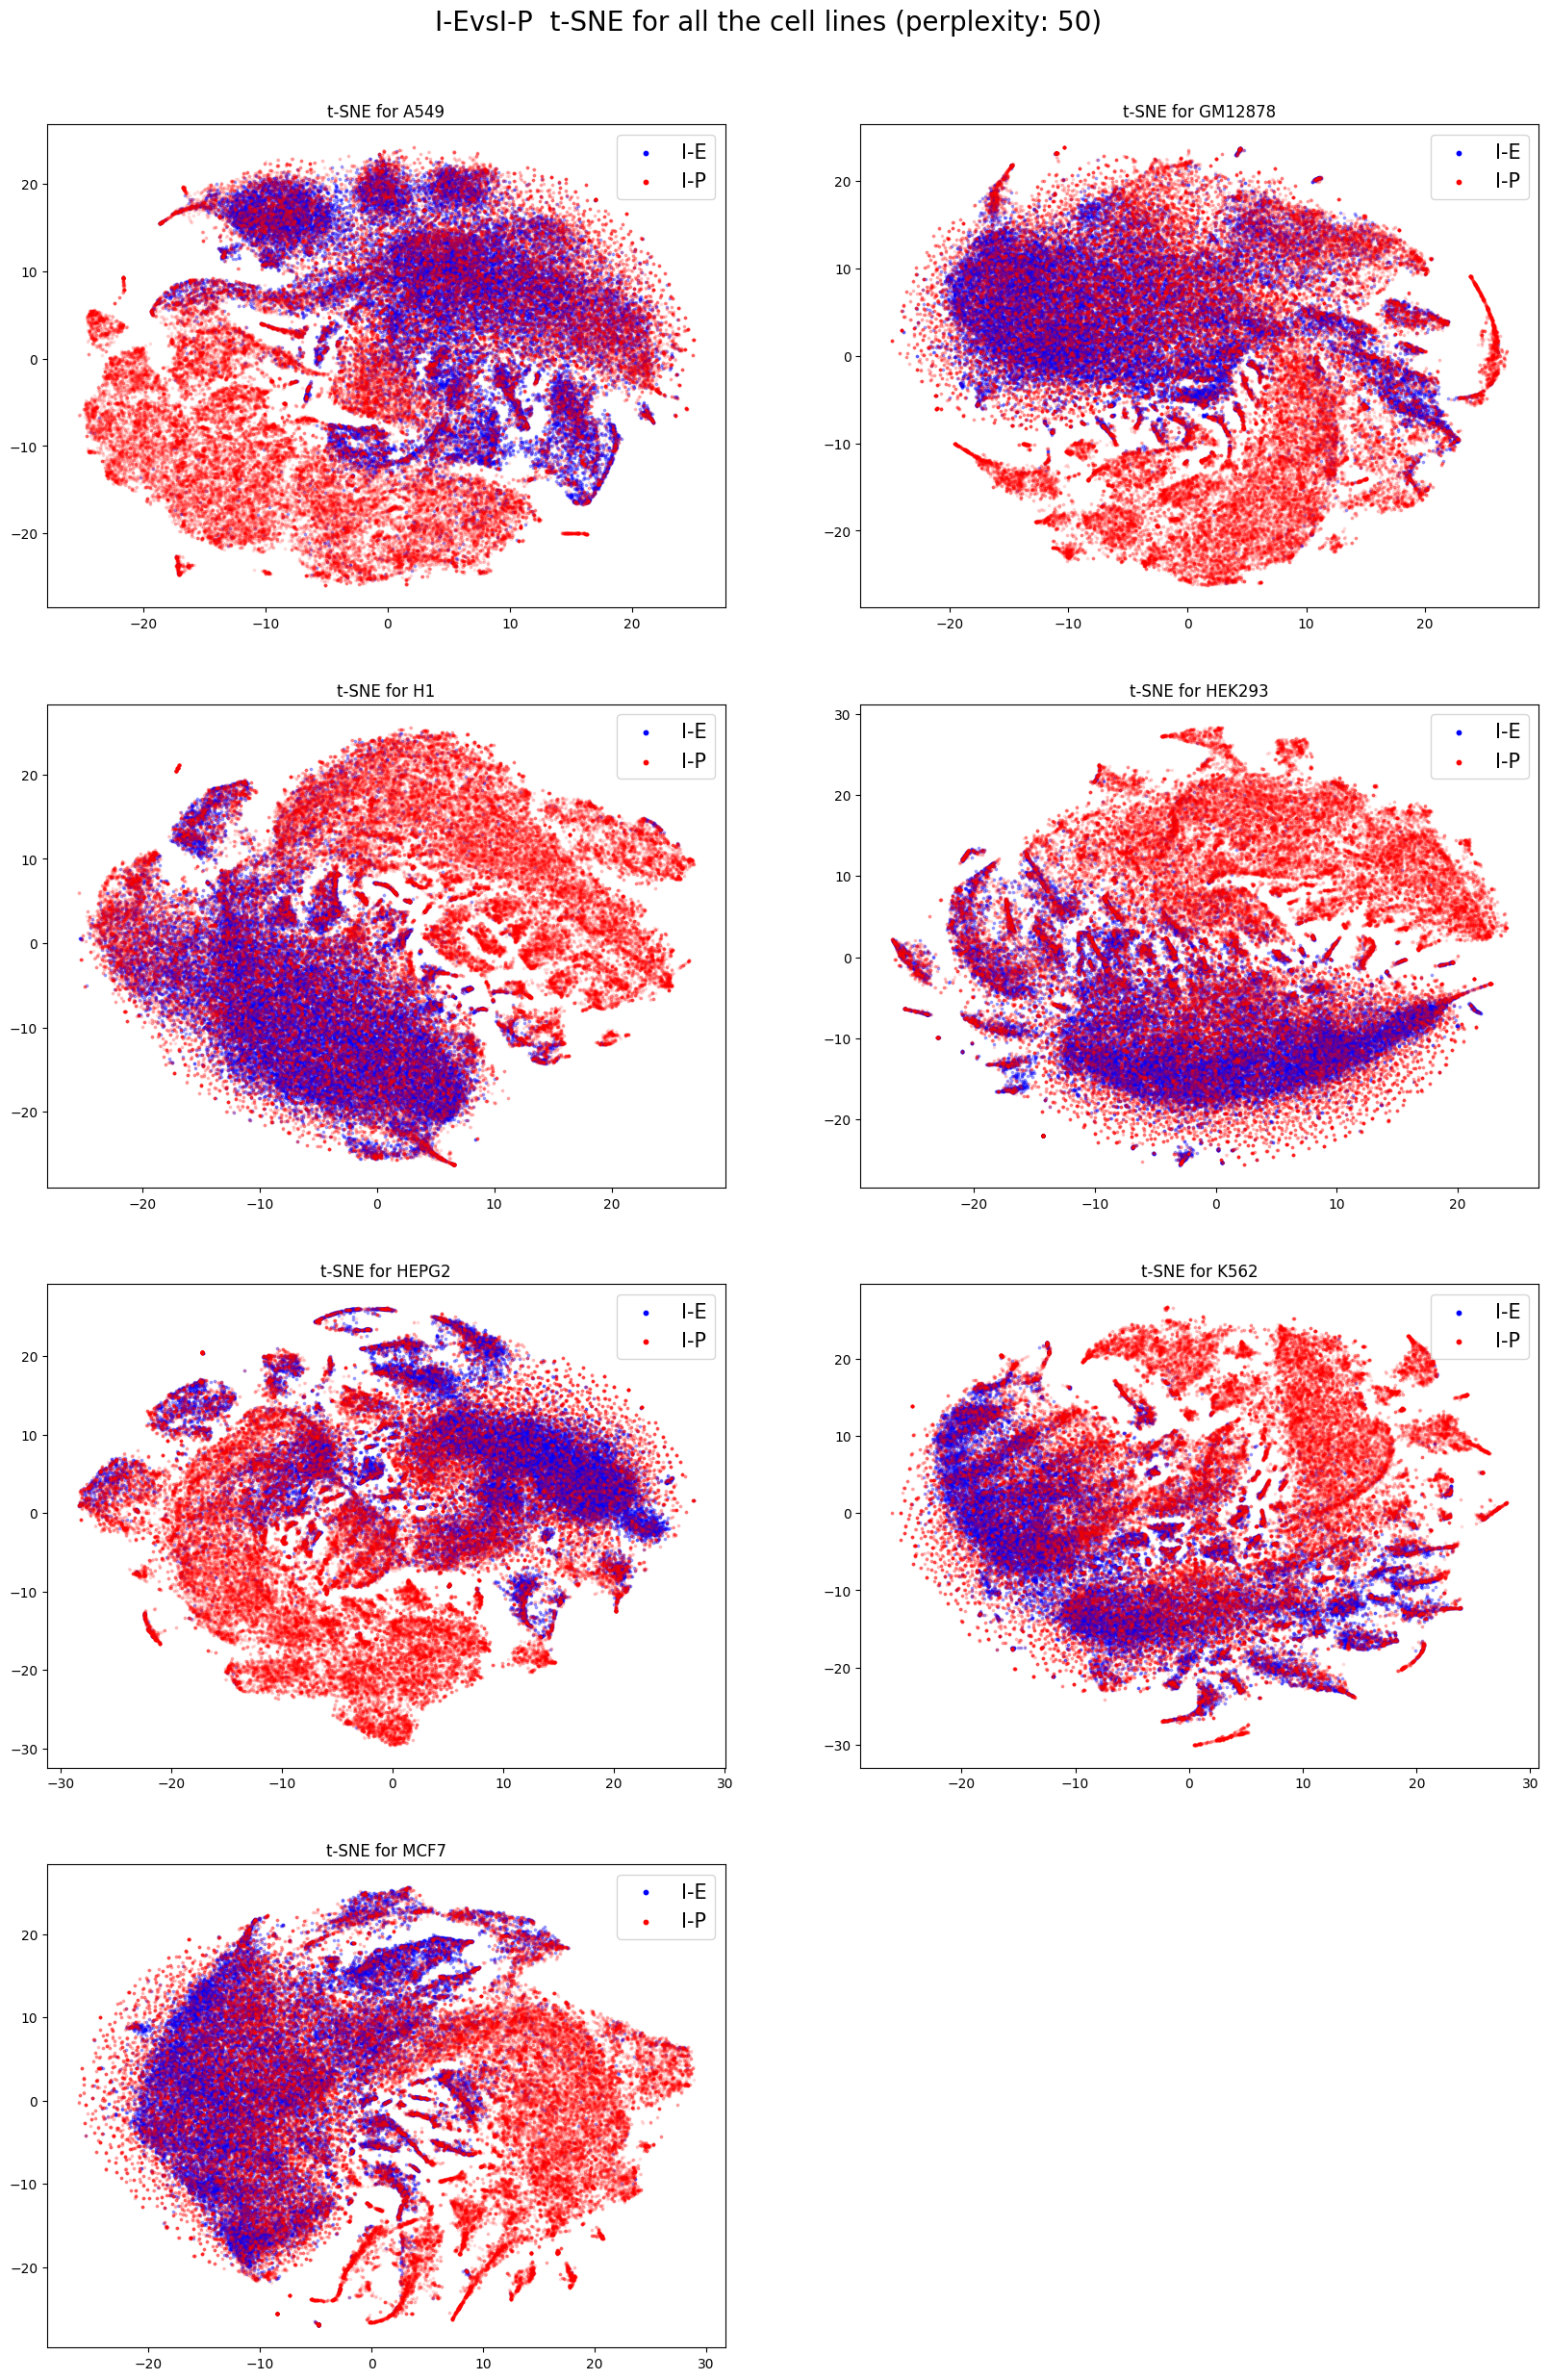
\includegraphics[width=12cm]{images/tsne_decomp_plots/20200410-232553_I-EvsI-P_tsne_plot.png}
\caption{t-SNE for I-E vs I-P}
\label{fig:tsneIEvsIP}
\end{figure}

\begin{figure}[h]
\centering
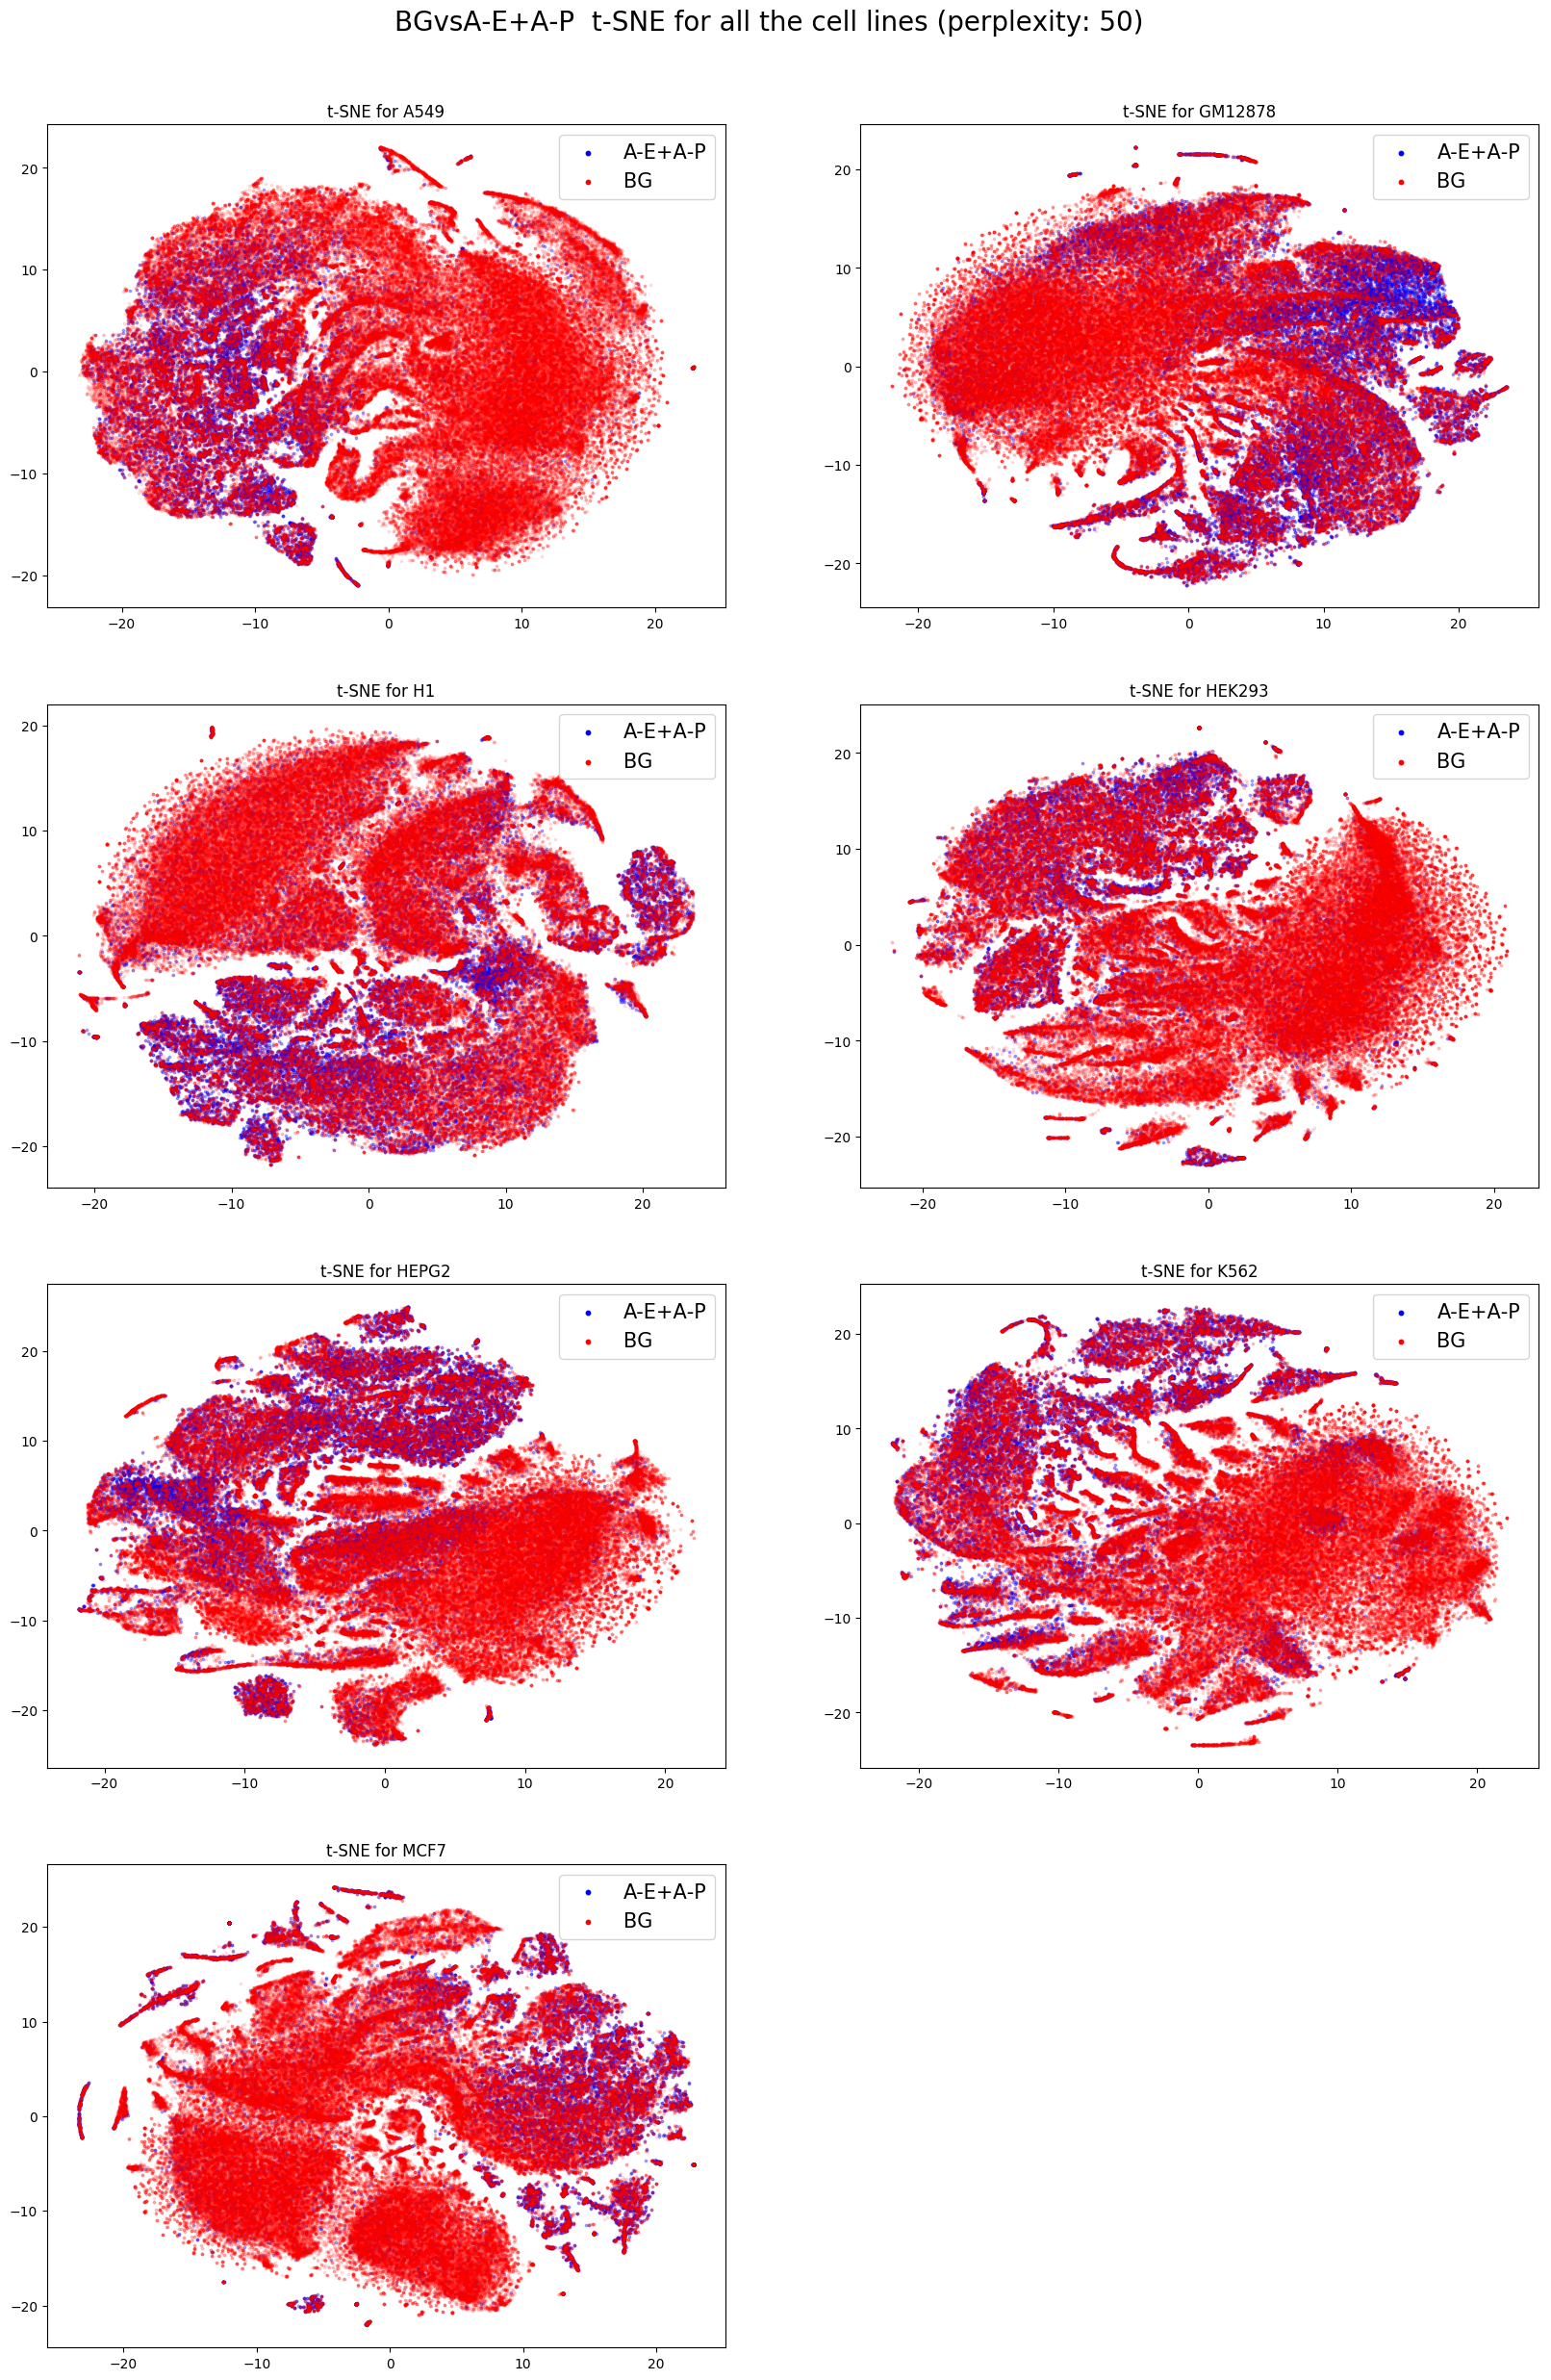
\includegraphics[width=12cm]{images/tsne_decomp_plots/20200410-232607_BGvsA-E+A-P_tsne_plot.png}
\caption{t-SNE for A-E+A-P vs BG}
\label{fig:tsneAE+APvsBG}
\end{figure}

\chapter{Features Importance Tables} \label{appendix:features_tables}
\begin{longtable}{lr}
\caption{}\\
\toprule
Features &  Score \\
\midrule
\endhead
\midrule
\multicolumn{2}{r}{{Continued on next page}} \\
\midrule
\endfoot

\bottomrule
\endlastfoot
    TAF1 &   4.00 \\
   SIN3A &   4.00 \\
 H3K4me2 &   3.20 \\
 H3K27ac &   3.20 \\
   H2AFZ &   3.00 \\
     YY1 &   2.40 \\
    PHF8 &   2.40 \\
     SP1 &   2.20 \\
    JUND &   2.00 \\
    ELF1 &   2.00 \\
 H3K4me3 &   2.00 \\
     MAZ &   1.80 \\
    RNF2 &   1.80 \\
    REST &   1.60 \\
    CHD4 &   1.40 \\
    USF2 &   1.40 \\
   TCF12 &   1.25 \\
   CEBPB &   1.20 \\
 ZC3H11A &   1.20 \\
    SIX5 &   1.20 \\
   FOSL2 &   1.20 \\
    CBX8 &   1.20 \\
    BCL3 &   1.20 \\
  ZBTB33 &   1.00 \\
   HDAC2 &   1.00 \\
    ETS1 &   1.00 \\
   KDM5A &   0.80 \\
    MAFK &   0.80 \\
  NFE2L2 &   0.80 \\
    CTCF &   0.60 \\
 H3K9me3 &   0.60 \\
   RCOR1 &   0.40 \\
   NR3C1 &   0.40 \\
    CBX2 &   0.40 \\
    SMC3 &   0.40 \\
  REST.1 &   0.40 \\
   KDM1A &   0.40 \\
   EHMT2 &   0.40 \\
  SREBF2 &   0.20 \\
    ATF3 &   0.20 \\
   ZFP36 &   0.20 \\
 NR3C1.1 &   0.20 \\
\end{longtable}

\begin{longtable}{lr}
\caption{GM12878 features}\\
\toprule
        Features &     Score \\
\midrule
\endhead
\midrule
\multicolumn{2}{r}{{Continued on next page}} \\
\midrule
\endfoot

\bottomrule
\endlastfoot
            TAF1 &  4.000000 \\
             TBP &  4.000000 \\
 POLR2AphosphoS5 &  4.000000 \\
          POLR2A &  4.000000 \\
          ZNF687 &  3.800000 \\
             RB1 &  3.500000 \\
             NBN &  3.400000 \\
            RELB &  3.000000 \\
            HDGF &  2.800000 \\
            ELF1 &  2.800000 \\
             YY1 &  2.800000 \\
 POLR2AphosphoS2 &  2.800000 \\
          STAT5A &  2.800000 \\
            NFIC &  2.750000 \\
           LARP7 &  2.666667 \\
         H3K4me3 &  2.600000 \\
            PAX8 &  2.600000 \\
          ETV6.1 &  2.400000 \\
           ZBED1 &  2.400000 \\
            E2F8 &  2.400000 \\
           ASH2L &  2.400000 \\
           FOXK2 &  2.333333 \\
           SIN3A &  2.200000 \\
          ZNF622 &  2.200000 \\
          WRNIP1 &  2.200000 \\
            UBTF &  2.200000 \\
         GATAD2B &  2.200000 \\
            CHD4 &  2.200000 \\
          BCL11A &  2.000000 \\
            BATF &  2.000000 \\
          NFATC1 &  2.000000 \\
           HCFC1 &  2.000000 \\
           SMAD5 &  2.000000 \\
         SMARCA5 &  2.000000 \\
             EED &  2.000000 \\
           IKZF2 &  2.000000 \\
            YBX1 &  1.800000 \\
           RUNX3 &  1.800000 \\
           MLLT1 &  1.800000 \\
             MAZ &  1.800000 \\
            IRF3 &  1.800000 \\
            NRF1 &  1.800000 \\
            CBFB &  1.800000 \\
            DPF2 &  1.600000 \\
           NFXL1 &  1.600000 \\
        TARDBP.1 &  1.600000 \\
           TBX21 &  1.600000 \\
           HDAC2 &  1.400000 \\
          TARDBP &  1.400000 \\
            NKRF &  1.400000 \\
            IRF5 &  1.400000 \\
            CREM &  1.400000 \\
            ATF2 &  1.200000 \\
           STAT3 &  1.200000 \\
             SRF &  1.200000 \\
            MTA2 &  1.200000 \\
            ATF7 &  1.200000 \\
          TRIM22 &  1.200000 \\
         BHLHE40 &  1.200000 \\
          BCLAF1 &  1.000000 \\
          ZNF207 &  1.000000 \\
            EBF1 &  1.000000 \\
            ETV6 &  1.000000 \\
           BACH1 &  1.000000 \\
           CEBPB &  1.000000 \\
            KLF5 &  1.000000 \\
            CBX5 &  1.000000 \\
            IRF4 &  1.000000 \\
         ZSCAN29 &  1.000000 \\
            PAX5 &  1.000000 \\
           RBBP5 &  1.000000 \\
           SMAD1 &  1.000000 \\
           STAT1 &  1.000000 \\
            E4F1 &  0.800000 \\
           RAD51 &  0.800000 \\
          PKNOX1 &  0.800000 \\
          ZNF592 &  0.800000 \\
          ARID3A &  0.800000 \\
          ZNF217 &  0.800000 \\
            ARNT &  0.600000 \\
           KDM1A &  0.600000 \\
           ZNF24 &  0.600000 \\
             MYB &  0.600000 \\
          ZBTB40 &  0.600000 \\
            TCF7 &  0.600000 \\
           RCOR1 &  0.600000 \\
           GABPA &  0.600000 \\
            JUNB &  0.600000 \\
            CBX3 &  0.600000 \\
            BMI1 &  0.600000 \\
          ZNF143 &  0.400000 \\
            HSF1 &  0.400000 \\
           CEBPZ &  0.400000 \\
            E2F4 &  0.400000 \\
            ETS1 &  0.400000 \\
           NR2F1 &  0.400000 \\
           NR2C1 &  0.200000 \\
            RFX5 &  0.200000 \\
            SMC3 &  0.200000 \\
\end{longtable}

\begin{longtable}{lr}
\caption{}\\
\toprule
  Features &  Score \\
\midrule
\endhead
\midrule
\multicolumn{2}{r}{{Continued on next page}} \\
\midrule
\endfoot

\bottomrule
\endlastfoot
    POLR2A &    4.0 \\
      PHF8 &    3.6 \\
       TBP &    3.6 \\
       SP1 &    3.6 \\
      TAF7 &    3.2 \\
      CHD2 &    3.0 \\
     SIN3A &    3.0 \\
   H3K27ac &    2.8 \\
   H3K4me3 &    2.8 \\
     HDAC2 &    2.8 \\
     KDM5A &    2.8 \\
       YY1 &    2.8 \\
 H2BK120ac &    2.4 \\
     RBBP5 &    2.4 \\
   H2BK5ac &    2.2 \\
      CBX8 &    2.2 \\
      TAF1 &    2.0 \\
      NRF1 &    2.0 \\
      JUND &    1.8 \\
       JUN &    1.8 \\
     EP300 &    1.8 \\
      CBX5 &    1.6 \\
      SIX5 &    1.6 \\
    H3K9ac &    1.6 \\
   H2AK5ac &    1.4 \\
     KDM1A &    1.4 \\
     H2AFZ &    1.4 \\
  H3K23me2 &    1.2 \\
  H2BK12ac &    1.2 \\
     RAD21 &    0.8 \\
      EGR1 &    0.6 \\
  H3K79me1 &    0.4 \\
      USF2 &    0.4 \\
      REST &    0.2 \\
\end{longtable}

\begin{longtable}{lr}
\caption{HEK293 features}\\
\toprule
     Features &  Score \\
\midrule
\endhead
\midrule
\multicolumn{2}{r}{{Continued on next page}} \\
\midrule
\endfoot

\bottomrule
\endlastfoot
     eGFP-SP2 &    4.0 \\
    eGFP-ZXDB &    3.2 \\
      H3K4me3 &    3.2 \\
    eGFP-KLF8 &    3.2 \\
  eGFP-ZNF335 &    3.2 \\
     eGFP-SP7 &    3.0 \\
      ZSCAN30 &    3.0 \\
       ZNF660 &    2.8 \\
 eGFP-ZNF518A &    2.8 \\
   eGFP-ZNF76 &    2.8 \\
     eGFP-SP3 &    2.8 \\
  eGFP-ZBTB26 &    2.6 \\
     eGFP-MAZ &    2.5 \\
     eGFP-YY2 &    2.4 \\
       ZNF561 &    2.4 \\
  eGFP-ZBTB11 &    2.2 \\
  eGFP-ZNF837 &    2.2 \\
  eGFP-ZNF639 &    2.0 \\
  eGFP-ZNF580 &    2.0 \\
  eGFP-ZBTB17 &    2.0 \\
    eGFP-ZNF2 &    2.0 \\
        ZFHX2 &    2.0 \\
    eGFP-KLF9 &    1.8 \\
  eGFP-ZNF202 &    1.8 \\
       ZNF195 &    1.8 \\
  eGFP-ZNF830 &    1.8 \\
       TRIM28 &    1.8 \\
   eGFP-PATZ1 &    1.8 \\
  eGFP-ZNF596 &    1.6 \\
  eGFP-BCL11B &    1.6 \\
   eGFP-TSHZ1 &    1.6 \\
         GLI2 &    1.6 \\
    eGFP-ZEB2 &    1.6 \\
   eGFP-KLF17 &    1.4 \\
  eGFP-ZNF362 &    1.4 \\
    eGFP-ZIC2 &    1.4 \\
  eGFP-ZNF777 &    1.4 \\
        ZNF26 &    1.4 \\
  eGFP-ZNF610 &    1.4 \\
   eGFP-GLIS2 &    1.4 \\
   eGFP-IKZF3 &    1.4 \\
   eGFP-KLF13 &    1.2 \\
   eGFP-KLF14 &    1.2 \\
   eGFP-PRDM1 &    1.2 \\
        PRDM6 &    1.2 \\
    eGFP-REST &    1.2 \\
  eGFP-ZNF600 &    1.2 \\
  eGFP-ZBTB20 &    1.2 \\
   eGFP-ZNF48 &    1.2 \\
  eGFP-ZNF843 &    1.2 \\
  eGFP-ZSCAN4 &    1.0 \\
  eGFP-ZNF501 &    1.0 \\
  eGFP-ZNF324 &    1.0 \\
  eGFP-ZNF391 &    1.0 \\
    eGFP-RBAK &    1.0 \\
       ZNF524 &    1.0 \\
    eGFP-KLF7 &    1.0 \\
   eGFP-KLF16 &    1.0 \\
        ZNF34 &    1.0 \\
  eGFP-ZNF121 &    1.0 \\
  eGFP-ZBTB10 &    0.8 \\
  eGFP-ZNF214 &    0.8 \\
   eGFP-ZNF24 &    0.8 \\
  eGFP-ZBTB7A &    0.8 \\
  eGFP-ZBTB49 &    0.8 \\
    eGFP-KLF1 &    0.8 \\
  eGFP-ZNF341 &    0.8 \\
  eGFP-ZNF654 &    0.8 \\
       ZBTB8A &    0.8 \\
  eGFP-ZNF785 &    0.8 \\
       ZNF366 &    0.8 \\
       ZNF555 &    0.8 \\
  eGFP-ZNF677 &    0.8 \\
   eGFP-INSM2 &    0.8 \\
  eGFP-ZNF558 &    0.8 \\
  eGFP-BCL11A &    0.6 \\
   eGFP-OVOL3 &    0.6 \\
       ZNF213 &    0.6 \\
       ZNF184 &    0.6 \\
    eGFP-ZEB1 &    0.6 \\
   eGFP-ZFP37 &    0.6 \\
   eGFP-KLF10 &    0.6 \\
  eGFP-ZNF101 &    0.6 \\
   eGFP-ZBTB6 &    0.6 \\
  eGFP-ZNF398 &    0.6 \\
  eGFP-ZNF770 &    0.6 \\
  eGFP-ZNF529 &    0.6 \\
  eGFP-ZNF513 &    0.6 \\
   eGFP-ZNF18 &    0.6 \\
  eGFP-ZNF473 &    0.6 \\
  eGFP-ZNF423 &    0.4 \\
  eGFP-ZNF449 &    0.4 \\
  eGFP-ZNF331 &    0.4 \\
       ZNF169 &    0.4 \\
  eGFP-REPIN1 &    0.4 \\
  eGFP-PRDM12 &    0.4 \\
    eGFP-OSR2 &    0.4 \\
  eGFP-ZNF791 &    0.4 \\
    eGFP-MYNN &    0.4 \\
  eGFP-ZNF692 &    0.4 \\
   eGFP-GLIS1 &    0.4 \\
       ZNF510 &    0.4 \\
   eGFP-FEZF1 &    0.4 \\
   eGFP-AEBP2 &    0.4 \\
   eGFP-ZBTB1 &    0.4 \\
       ZNF658 &    0.4 \\
 eGFP-ZSCAN5A &    0.4 \\
  eGFP-ZNF132 &    0.4 \\
  eGFP-ZNF239 &    0.4 \\
  eGFP-ZNF157 &    0.4 \\
       ZBTB44 &    0.4 \\
  eGFP-ZNF114 &    0.4 \\
  eGFP-ZNF112 &    0.4 \\
        BCL6B &    0.4 \\
        SALL2 &    0.4 \\
 eGFP-ZSCAN21 &    0.4 \\
 eGFP-ZNF280C &    0.2 \\
  eGFP-PRDM10 &    0.2 \\
       ZNF560 &    0.2 \\
      ZSCAN26 &    0.2 \\
  eGFP-ZNF626 &    0.2 \\
  eGFP-ZNF521 &    0.2 \\
  eGFP-ZNF493 &    0.2 \\
 eGFP-ZSCAN5C &    0.2 \\
   eGFP-SCRT2 &    0.2 \\
       ZBTB48 &    0.2 \\
       ZNF571 &    0.2 \\
     eGFP-WT1 &    0.2 \\
\end{longtable}

\begin{longtable}{lr}
\caption{HEPG2 features}\\
\toprule
        Features &     Score \\
\midrule
\endhead
\midrule
\multicolumn{2}{r}{{Continued on next page}} \\
\midrule
\endfoot

\bottomrule
\endlastfoot
          POLR2G &  4.000000 \\
 POLR2AphosphoS5 &  4.000000 \\
          RBFOX2 &  4.000000 \\
    3xFLAG-DRAP1 &  3.200000 \\
     3xFLAG-MBD1 &  3.000000 \\
            AGO2 &  3.000000 \\
         H3K4me3 &  2.600000 \\
         H3K4me2 &  2.500000 \\
           KDM1A &  2.400000 \\
   3xFLAG-GATAD1 &  2.250000 \\
            EZH2 &  2.200000 \\
           SIN3A &  2.200000 \\
    3xFLAG-HOMEZ &  2.000000 \\
             TBP &  2.000000 \\
            TAF1 &  1.800000 \\
    3xFLAG-TFDP1 &  1.800000 \\
           RBM22 &  1.800000 \\
     3xFLAG-TFE3 &  1.666667 \\
    3xFLAG-TGIF2 &  1.666667 \\
           KDM3A &  1.600000 \\
  3xFLAG-ZKSCAN8 &  1.400000 \\
            ETV5 &  1.400000 \\
          DNMT3B &  1.400000 \\
    3xFLAG-SSRP1 &  1.400000 \\
     3xFLAG-HHEX &  1.200000 \\
     3xFLAG-PAF1 &  1.200000 \\
           HCFC1 &  1.200000 \\
    3xFLAG-MIER2 &  1.200000 \\
           XRCC5 &  1.200000 \\
     3xFLAG-SOX5 &  1.000000 \\
     3xFLAG-HBP1 &  1.000000 \\
     3xFLAG-KLF9 &  1.000000 \\
   3xFLAG-THAP11 &  1.000000 \\
          ZBTB25 &  1.000000 \\
    3xFLAG-GMEB2 &  1.000000 \\
             MAZ &  1.000000 \\
          TARDBP &  1.000000 \\
            BRD4 &  1.000000 \\
    3xFLAG-ZNF48 &  1.000000 \\
    3xFLAG-TEAD3 &  1.000000 \\
           PLRG1 &  1.000000 \\
          HMG20B &  1.000000 \\
           SIN3B &  0.800000 \\
           CCAR2 &  0.800000 \\
        GTF2F1.1 &  0.800000 \\
         SMARCE1 &  0.800000 \\
           PCBP1 &  0.800000 \\
          ZBTB7A &  0.800000 \\
            RARA &  0.800000 \\
            ETS1 &  0.800000 \\
           ZNF24 &  0.800000 \\
    3xFLAG-FOXA3 &  0.750000 \\
           PPARG &  0.600000 \\
             FUS &  0.600000 \\
           RCOR1 &  0.600000 \\
    3xFLAG-CREB1 &  0.600000 \\
         TBL1XR1 &  0.600000 \\
      3xFLAG-SP5 &  0.600000 \\
            NRF1 &  0.600000 \\
          BCLAF1 &  0.600000 \\
            YBX1 &  0.600000 \\
         SNRNP70 &  0.600000 \\
   3xFLAG-ZBTB26 &  0.500000 \\
          ZNF205 &  0.500000 \\
          ZNF644 &  0.400000 \\
           GATA4 &  0.400000 \\
           FOSL2 &  0.400000 \\
     3xFLAG-THRB &  0.400000 \\
           CREB1 &  0.400000 \\
           BRCA1 &  0.400000 \\
            ATF3 &  0.400000 \\
            ARNT &  0.400000 \\
         HNRNPH1 &  0.400000 \\
            PBX2 &  0.400000 \\
     3xFLAG-ZNF7 &  0.400000 \\
           SRSF1 &  0.400000 \\
 POLR2AphosphoS2 &  0.400000 \\
           NR2F6 &  0.400000 \\
            NONO &  0.400000 \\
            RNF2 &  0.400000 \\
         SMARCC2 &  0.400000 \\
    3xFLAG-KDM6A &  0.400000 \\
             MNT &  0.400000 \\
           LCORL &  0.400000 \\
    3xFLAG-NR2F1 &  0.400000 \\
            ZHX2 &  0.400000 \\
           FOXP1 &  0.200000 \\
            TOE1 &  0.200000 \\
           FOXA2 &  0.200000 \\
           U2AF1 &  0.200000 \\
           CEBPB &  0.200000 \\
            JUND &  0.200000 \\
             HLF &  0.200000 \\
         H3K9me3 &  0.200000 \\
           NFRKB &  0.200000 \\
      3xFLAG-MLX &  0.200000 \\
    3xFLAG-NFIL3 &  0.200000 \\
            NFYC &  0.200000 \\
\end{longtable}

\begin{longtable}{lr}
\caption{K562 features}\\
\toprule
        Features &     Score \\
\midrule
\endhead
\midrule
\multicolumn{2}{r}{{Continued on next page}} \\
\midrule
\endfoot

\bottomrule
\endlastfoot
          SUPT5H &  4.000000 \\
           SMAD5 &  4.000000 \\
             TBP &  3.800000 \\
             PML &  3.200000 \\
          RBFOX2 &  3.000000 \\
 POLR2AphosphoS2 &  3.000000 \\
          H3K9ac &  2.800000 \\
           H2AFZ &  2.800000 \\
           EP400 &  2.600000 \\
            BRD4 &  2.400000 \\
           SIN3A &  2.400000 \\
          POLR2A &  2.000000 \\
             RB1 &  2.000000 \\
           BRCA1 &  2.000000 \\
           MNT.2 &  2.000000 \\
            MBD2 &  2.000000 \\
             MAX &  2.000000 \\
         H3K4me3 &  2.000000 \\
          ZNF592 &  1.800000 \\
           TAF9B &  1.800000 \\
            CREM &  1.800000 \\
           HCFC1 &  1.800000 \\
           TAF15 &  1.800000 \\
            HDGF &  1.800000 \\
          RNF2.1 &  1.750000 \\
         TBL1XR1 &  1.600000 \\
            MCM5 &  1.600000 \\
            MCM3 &  1.600000 \\
            IRF1 &  1.600000 \\
           VEZF1 &  1.600000 \\
      eGFP-FOSL1 &  1.600000 \\
          GTF2F1 &  1.400000 \\
            NKRF &  1.400000 \\
            NRF1 &  1.400000 \\
            ZZZ3 &  1.400000 \\
            MTA3 &  1.400000 \\
           COPS2 &  1.400000 \\
           TCF12 &  1.333333 \\
             ZFX &  1.200000 \\
          ZBTB33 &  1.200000 \\
            MXI1 &  1.200000 \\
             NBN &  1.200000 \\
            TAF7 &  1.200000 \\
             SP1 &  1.200000 \\
           PTBP1 &  1.200000 \\
            ILF3 &  1.200000 \\
           EWSR1 &  1.200000 \\
            AFF1 &  1.200000 \\
            AGO1 &  1.200000 \\
           SIN3B &  1.000000 \\
            ATF3 &  1.000000 \\
          TRIM24 &  1.000000 \\
          RNF2.3 &  1.000000 \\
     eGFP-POLR2H &  1.000000 \\
           SMAD1 &  1.000000 \\
          STAT5A &  1.000000 \\
          ARID1B &  1.000000 \\
            ELF4 &  1.000000 \\
           SRSF1 &  1.000000 \\
          MCM2.1 &  1.000000 \\
           CTBP1 &  1.000000 \\
      eGFP-KLF13 &  1.000000 \\
         SMARCA5 &  1.000000 \\
            UBTF &  0.800000 \\
            JUND &  0.800000 \\
     eGFP-ZNF512 &  0.800000 \\
            MCM2 &  0.800000 \\
            CBX3 &  0.800000 \\
           KDM1A &  0.800000 \\
        CHAMP1.1 &  0.800000 \\
            SFPQ &  0.800000 \\
          POU5F1 &  0.800000 \\
       eGFP-RELA &  0.800000 \\
           SRSF7 &  0.800000 \\
            LEF1 &  0.800000 \\
          LEF1.1 &  0.800000 \\
     3xFLAG-ATF1 &  0.800000 \\
     3xFLAG-PBX2 &  0.800000 \\
          ARNT.1 &  0.800000 \\
            BRD9 &  0.800000 \\
         NEUROD1 &  0.800000 \\
         ZC3H11A &  0.800000 \\
           FOXA1 &  0.800000 \\
           ZMIZ1 &  0.800000 \\
        C11orf30 &  0.800000 \\
           EP300 &  0.750000 \\
           ZBTB2 &  0.600000 \\
            RNF2 &  0.600000 \\
      eGFP-TFDP1 &  0.600000 \\
      eGFP-MEF2D &  0.600000 \\
             FUS &  0.600000 \\
           GABPA &  0.600000 \\
         ZKSCAN8 &  0.600000 \\
          RNF2.2 &  0.600000 \\
           RUNX1 &  0.600000 \\
           PHF20 &  0.600000 \\
            REST &  0.600000 \\
            ZHX1 &  0.600000 \\
          CC2D1A &  0.500000 \\
         SMARCA4 &  0.500000 \\
           NCOA1 &  0.400000 \\
            PHB2 &  0.400000 \\
            MTA2 &  0.400000 \\
         SMARCC2 &  0.400000 \\
           FOXM1 &  0.400000 \\
           ESRRA &  0.400000 \\
           NFRKB &  0.400000 \\
            DPF2 &  0.400000 \\
           DNMT1 &  0.400000 \\
          NUFIP1 &  0.400000 \\
            NONO &  0.400000 \\
            E4F1 &  0.400000 \\
            SKIL &  0.400000 \\
     eGFP-ZNF584 &  0.400000 \\
            RFX1 &  0.400000 \\
             RLF &  0.400000 \\
       eGFP-ADNP &  0.400000 \\
           LARP7 &  0.400000 \\
      eGFP-DIDO1 &  0.400000 \\
          CHAMP1 &  0.400000 \\
           ASH1L &  0.400000 \\
          ZNF407 &  0.400000 \\
        HNRNPUL1 &  0.400000 \\
          ZNF184 &  0.400000 \\
            ARNT &  0.400000 \\
           ZFP91 &  0.400000 \\
           ZBTB5 &  0.400000 \\
     eGFP-ZNF589 &  0.400000 \\
            CBX1 &  0.400000 \\
        GTF2F1.1 &  0.400000 \\
           CDC5L &  0.400000 \\
          THRAP3 &  0.400000 \\
     eGFP-GTF2A2 &  0.400000 \\
     eGFP-GTF2E2 &  0.400000 \\
          TARDBP &  0.400000 \\
           HDAC3 &  0.400000 \\
           SUZ12 &  0.400000 \\
           KHSRP &  0.400000 \\
      eGFP-FOXJ2 &  0.400000 \\
       eGFP-NFE2 &  0.250000 \\
       eGFP-MAFG &  0.250000 \\
             MNT &  0.200000 \\
          ZNF318 &  0.200000 \\
       eGFP-ATF1 &  0.200000 \\
             ID3 &  0.200000 \\
         ZSCAN29 &  0.200000 \\
           MLLT1 &  0.200000 \\
           IKZF1 &  0.200000 \\
      eGFP-BACH1 &  0.200000 \\
          HNRNPL &  0.200000 \\
           NCOA2 &  0.200000 \\
           FOXK2 &  0.200000 \\
       eGFP-ELF1 &  0.200000 \\
       eGFP-PTRF &  0.200000 \\
      eGFP-PTTG1 &  0.200000 \\
            MCM7 &  0.200000 \\
        ZBTB40.1 &  0.200000 \\
    eGFP-ZNF354B &  0.200000 \\
           SRSF9 &  0.200000 \\
            SAFB &  0.200000 \\
         CBFA2T3 &  0.200000 \\
           RBM17 &  0.200000 \\
           HDAC2 &  0.200000 \\
           CEBPG &  0.200000 \\
         GATAD2A &  0.200000 \\
\end{longtable}

\begin{longtable}{lr}
\caption{MCF7 features}\\
\toprule
   Features &  Score \\
\midrule
\endhead
\midrule
\multicolumn{2}{r}{{Continued on next page}} \\
\midrule
\endfoot

\bottomrule
\endlastfoot
        MYC &    4.0 \\
      SIN3A &    3.6 \\
     GTF2F1 &    3.6 \\
    H3K4me3 &    3.2 \\
       MBD2 &    3.0 \\
       CHD1 &    2.8 \\
        MAZ &    2.8 \\
    H3K27ac &    2.8 \\
       NRF1 &    2.6 \\
       ELF1 &    2.4 \\
       ZHX2 &    2.4 \\
  eGFP-KLF9 &    2.2 \\
      ZBTB1 &    2.0 \\
     ZNF592 &    2.0 \\
    H3K4me1 &    2.0 \\
        ZFX &    1.8 \\
     ZNF217 &    1.6 \\
       MTA3 &    1.6 \\
  eGFP-ELF1 &    1.6 \\
     ARID3A &    1.6 \\
     ZNF687 &    1.6 \\
    SMARCA5 &    1.4 \\
     TARDBP &    1.2 \\
       MTA2 &    1.2 \\
      FOXK2 &    1.2 \\
        FOS &    1.2 \\
      CLOCK &    1.0 \\
     ZBTB7B &    1.0 \\
      CTBP1 &    1.0 \\
      NFRKB &    0.8 \\
    H3K9me3 &    0.8 \\
       HDGF &    0.8 \\
       HES1 &    0.8 \\
       HSF1 &    0.8 \\
      GABPA &    0.8 \\
  ZNF512B.1 &    0.8 \\
        MNT &    0.8 \\
    ZKSCAN1 &    0.8 \\
       CUX1 &    0.8 \\
     ZNF444 &    0.8 \\
      CREB1 &    0.6 \\
       DPF2 &    0.6 \\
       MTA1 &    0.6 \\
       E4F1 &    0.6 \\
    NEUROD1 &    0.6 \\
       NFIB &    0.4 \\
     ZBTB33 &    0.4 \\
   ZNF217.1 &    0.4 \\
       E2F8 &    0.4 \\
       TOE1 &    0.4 \\
      SUZ12 &    0.4 \\
    PPP1R10 &    0.4 \\
    ZNF512B &    0.4 \\
    SMARCE1 &    0.4 \\
      NFXL1 &    0.2 \\
 eGFP-CEBPG &    0.2 \\
       ELK1 &    0.2 \\
      NCOA3 &    0.2 \\
 eGFP-FOSL2 &    0.2 \\
\end{longtable}


\printbibliography

\end{document}
